\RequirePackage[l2tabu, orthodox]{nag}

%\documentclass[]{article}
\documentclass[11pt]{scrartcl}
\usepackage[usename, dvipsnames]{xcolor}
\usepackage[pdfencoding=auto]{hyperref}
\usepackage[msc-links]{amsrefs}
\usepackage{cleveref} % use \cref{}, automatically deduces theorem, proposition, etc
\usepackage[mathletters]{ucs}
\usepackage[utf8]{inputenc}
\usepackage[T1]{fontenc}
\usepackage{datetime}

\usepackage{array}
\usepackage{mathtools}
\usepackage{amsmath, amsthm, amssymb, amsfonts, amsxtra, amscd, thmtools}
\let\proof\relax
\let\endproof\relax

% Boxes around theorem environments.
\usepackage[many]{tcolorbox}

\usepackage{color}
%\usepackage{unicode-math}
\usepackage{newunicodechar}
\newunicodechar{ε}{\varepsilon}
\newunicodechar{δ}{\delta}
\newunicodechar{µ}{\mu}
\newunicodechar{→}{\to}
\newunicodechar{≤}{\leq}
\newunicodechar{∈}{\in}
\newunicodechar{⊆}{\subseteq}
\newunicodechar{Λ}{\Lambda}
\newunicodechar{∞}{\infty}
\newunicodechar{×}{\times}
\everymath{\displaystyle}



\usepackage{microtype}
\usepackage[pdfencoding=auto]{hyperref}
\usepackage{bookmark}
\usepackage{booktabs}
\usepackage{todonotes}
\usepackage[msc-links]{amsrefs}
\usepackage{cleveref} % use \cref{}, automatically deduces theorem, proposition, etc
\usepackage{csquotes}
\usepackage{longtable}
\usepackage{tabularx}
\usepackage{bbm}
% Creating multiple types of index
\usepackage{imakeidx}

% Remove indentation for new paragraphs
\usepackage{parskip}
% But leave space before amsthm environments
\makeatletter
\def\thm@space@setup{%
  \thm@preskip=2em
  \thm@postskip=2em
}
\makeatother


\usepackage{stmaryrd}
\usepackage{adjustbox}
\usepackage{centernot}
% \centernot\whatever


% Better indicator function
\usepackage{bbm}
\newcommand{\indic}[1]{\mathbbm{1} \left[ {#1} \right] }

% Highlight quote
\usepackage{environ}
\definecolor{camel}{rgb}{0.76, 0.6, 0.42}
\definecolor{babyblue}{rgb}{0.54, 0.81, 0.94}
\definecolor{block-gray}{gray}{0.85}
\NewEnviron{myblock}
{\colorbox{block-gray}{%
\parbox{\dimexpr\linewidth-2\fboxsep\relax}{%
\small\addtolength{\leftskip}{10mm}
\addtolength{\rightskip}{10mm}
\BODY}}
}
\renewcommand{\quote}{\myblock}
\renewcommand{\endquote}{\endmyblock}

% Nice math font that journals use
%\usepackage[lite]{mtpro2}
%\usepackage{mathrsfs}
%\usepackage{mathptmx}
\usepackage{lmodern}
%\usepackage[sc]{mathpazo}

% Theorem Styles
\usepackage[framemethod=tikz]{mdframed}

\theoremstyle{definition}
\newtheorem{exercise}{Exercise}[section]
\newtheorem{solution}{Solution}

% Theorem Style
\newtheoremstyle{theorem}% name
  {0em}%         Space above, empty = `usual value'
  {1em}%         Space below
  {\normalfont}% Body font
  {\parindent}%         Indent amount (empty = no indent, \parindent = para indent)
  {\bfseries}% Thm head font
  {.}%        Punctuation after thm head
  {\newline}% Space after thm head: \newline = linebreak
  {\thmname{#1}\thmnumber{ #2}\thmnote{\itshape{(#3)}}}%
\theoremstyle{theorem}
\tcolorboxenvironment{theorem}{
  boxrule=0pt,
  boxsep=0pt,
  breakable,
  enhanced jigsaw,
  fonttitle={\large\bfseries},
  opacityback=0.8,
  colframe=cyan,
  borderline west={4pt}{0pt}{orange},
  attach title to upper={}
}
\newtheorem{theorem}{Theorem}[section]

% Proposition Style
\tcolorboxenvironment{proposition}{
  boxrule=1pt,
  boxsep=0pt,
  breakable,
  enhanced jigsaw,
  opacityback=0.0,
  colframe=cyan
}
\newtheorem{proposition}[theorem]{Proposition}
\tcolorboxenvironment{lemma}{
  boxrule=1pt,
  boxsep=0pt,
  breakable,
  enhanced jigsaw,
  opacityback=0.2,
  colframe=cyan
}
\newtheorem{lemma}[theorem]{Lemma}
% Claim
\tcolorboxenvironment{claim}{
  boxrule=1pt,
  boxsep=0pt,
  breakable,
  enhanced jigsaw,
  opacityback=0.2,
  colframe=cyan
}
\newtheorem{claim}[theorem]{Claim}


% Corollary
\tcolorboxenvironment{corollary}{
  colback=cyan,
  boxrule=1pt,
  boxsep=0pt,
  breakable,
  enhanced jigsaw,
  opacityback=0.1,
  colframe=cyan
}
\newtheorem{corollary}[theorem]{Corollary}

% Proof Style
\newtheoremstyle{proof}% name
  {0em}%         Space above, empty = `usual value'
  {2em}%         Space below
  {\normalfont}% Body font
  {\parindent}%         Indent amount (empty = no indent, \parindent = para indent)
  {\itshape}% Thm head font
  {.}%        Punctuation after thm head
  {\newline}% Space after thm head: \newline = linebreak
  {\thmname{#1} \thmnote{\itshape{(#3)}}}%         Thm head spec
\theoremstyle{proof}
\tcolorboxenvironment{proof}{
  colback=camel,
  opacityfill=0.25,
  boxrule=1pt,
  boxsep=0pt,
  breakable,
  enhanced jigsaw
}
\newtheorem*{pf}{Proof}
\newenvironment{proof}
{\pushQED{$\qed$}\pf}
{\par\popQED\endpf}

% Definition Style
\newtheoremstyle{definition}% name
  {0em}%         Space above, empty = `usual value'
  {2em}%         Space below
  {\normalfont}% Body font
  {\parindent}%         Indent amount (empty = no indent, \parindent = para indent)
  {\bfseries}% Thm head font
  {.}%        Punctuation after thm head
  {\newline}% Space after thm head: \newline = linebreak
  {}%         Thm head spec
\theoremstyle{definition}
\tcolorboxenvironment{definition}{
  colback=babyblue,
  boxrule=0pt,
  boxsep=0pt,
  opacityfill=0.45,
  breakable,
  enhanced jigsaw,
  borderline west={4pt}{0pt}{blue},
  colbacktitle={babyblue},
  coltitle={black},
  fonttitle={\large\bfseries},
  attach title to upper={},
}
\newtheorem{definition}{Definition}[theorem]

% Break Environment
\makeatletter
\newtheoremstyle{break}% name
  {}%         Space above, empty = `usual value'
  {2em}%         Space below
  {
    \addtolength{\@totalleftmargin}{2.5em}
    \addtolength{\linewidth}{-2.5em}
    \parshape 1 2.5em \linewidth
  }% Body font
  {}%         Indent amount (empty = no indent, \parindent = para indent)
  {\bfseries}% Thm head font
  {.}%        Punctuation after thm head
  {\newline}% Space after thm head: \newline = linebreak
  {}%         Thm head spec
\makeatother

\theoremstyle{break}
\newtheorem{example}{Example}[section]

% Problem Style
\newtheoremstyle{problem} % name
  {0em}                   % Space above, empty = `usual value'
  {2em}                   % Space below
  {\normalfont}           % Body font
  {\parindent}            % Indent amount (empty = no indent, \parindent = para indent)
  {\itshape}              % Thm head font
  {}                      % Punctuation after thm head
  {\newline}              % Space after thm head: \newline = linebreak
  {\thmnote{\itshape{(#3)}}}     % Thm head spec
\theoremstyle{problem}
\tcolorboxenvironment{problem}{
  boxrule=1pt,
  boxsep=0pt,
  breakable,
  enhanced jigsaw,
  opacityback=0.0,
  colframe=cyan
}
\newtheorem{problem}{Problem}


%Pagination stuff.
\setlength{\topmargin}{-.3 in}
\setlength{\oddsidemargin}{0in}
\setlength{\evensidemargin}{0in}
\setlength{\textheight}{9.in}
\setlength{\textwidth}{6.5in}
% \pagestyle{empty} %removes page numbers.

% Inkscape figures from Vim
\usepackage{import}
\usepackage{pdfpages}
\usepackage{transparent}

\newcommand{\incfig}[1]{%
    \def\svgwidth{\columnwidth}
    \import{./figures/}{#1.pdf_tex}
}
%\pdfsuppresswarningpagegroup=1

% Pandoc-specific fixes
\providecommand{\tightlist}{%
  \setlength{\itemsep}{0pt}\setlength{\parskip}{0pt}}

% Tikz and Graphics
\usepackage{amscd}
\usepackage{tikz}
\usetikzlibrary{arrows, arrows.meta, cd, fadings, patterns, calc, decorations.markings, matrix, positioning}
\tikzfading[name=fade out, inner color=transparent!0, outer color=transparent!100]
\usepackage{pgfplots}
\pgfplotsset{compat=1.16}
\usepackage[inline]{asymptote}
\usepackage{tikz-layers}

%\usepackage{nath}
%\delimgrowth=1
\DeclarePairedDelimiter\qty{(}{)}

% Major Macros
\usepackage{graphicx}
\usepackage{float}
\DeclareFontFamily{U}{mathx}{\hyphenchar\font45}
\DeclareFontShape{U}{mathx}{m}{n}{
      <5> <6> <7> <8> <9> <10>
      <10.95> <12> <14.4> <17.28> <20.74> <24.88>
      mathx10
      }{}
\DeclareSymbolFont{mathx}{U}{mathx}{m}{n}
\DeclareMathSymbol{\bigtimes}{1}{mathx}{"91}

% Wide tikz equations
\newsavebox{\wideeqbox}
\newenvironment{wideeq}
  {\begin{displaymath}\begin{lrbox}{\wideeqbox}$\displaystyle}
  {$\end{lrbox}\makebox[0pt]{\usebox{\wideeqbox}}\end{displaymath}}



% Fancy chapter headers and footers
\usepackage{fancyhdr}

\pagestyle{fancy}
\fancyhf{}
\fancyhead[LE,RO]{\title}
\fancyhead[RE,LO]{\rightmark}
\fancyfoot[CE,CO]{\leftmark}
\fancyfoot[LE,RO]{\thepage}

\renewcommand{\headrulewidth}{2pt}
\renewcommand{\footrulewidth}{1pt}

% List of Theorems Attempt
\usepackage{etoolbox}
\makeatletter
\patchcmd\thmtlo@chaptervspacehack
  {\addtocontents{loe}{\protect\addvspace{10\p@}}}
  {\addtocontents{loe}{\protect\thmlopatch@endchapter\protect\thmlopatch@chapter{\thechapter}}}
  {}{}
\AtEndDocument{\addtocontents{loe}{\protect\thmlopatch@endchapter}}
\long\def\thmlopatch@chapter#1#2\thmlopatch@endchapter{%
  \setbox\z@=\vbox{#2}%
  \ifdim\ht\z@>\z@
    \hbox{\bfseries\chaptername\ #1}\nobreak
    #2
    \addvspace{10\p@}
  \fi
}
\def\thmlopatch@endchapter{}

\makeatother
\renewcommand{\thmtformatoptarg}[1]{ -- #1}
%\renewcommand{\listtheoremname}{List of definitions}

\newcommand{\ext}{\operatorname{Ext}}
\newcommand{\Ext}{\operatorname{Ext}}
\def\Endo{\operatorname{End}}
\def\Ind{\operatorname{Ind}}
\def\ind{\operatorname{Ind}}
\def\coind{\operatorname{Coind}}
\def\Res{\operatorname{Res}}
\def\Hol{\operatorname{Hol}}
\def\res{\operatorname{Res}}
\def\endo{\operatorname{End}}
\def\ind{\operatorname{Ind}}
\renewcommand{\AA}[0]{{\mathbb{A}}}
\DeclareMathOperator{\Exists}{\exists}
\DeclareMathOperator{\Forall}{\forall}
\newcommand{\Af}[0]{{\mathbb{A}}}
\newcommand{\CC}[0]{{\mathbb{C}}}
\newcommand{\CP}[0]{{\mathbb{CP}}}
\newcommand{\DD}[0]{{\mathbb{D}}}
\newcommand{\FF}[0]{{\mathbb{F}}}
\newcommand{\GF}[0]{{\mathbb{GF}}}
\newcommand{\GG}[0]{{\mathbb{G}}}
\newcommand{\HH}[0]{{\mathbb{H}}}
\newcommand{\HP}[0]{{\mathbb{HP}}}
\newcommand{\KK}[0]{{\mathbb{K}}}
\newcommand{\kk}[0]{{\Bbbk}}
\newcommand{\bbm}[0]{{\mathbb{M}}}
\newcommand{\NN}[0]{{\mathbb{N}}}
\newcommand{\OP}[0]{{\mathbb{OP}}}
\newcommand{\PP}[0]{{\mathbb{P}}}
\newcommand{\QQ}[0]{{\mathbb{Q}}}
\newcommand{\RP}[0]{{\mathbb{RP}}}
\newcommand{\RR}[0]{{\mathbb{R}}}
\newcommand{\SpSp}[0]{{\mathbb{S}}}
\renewcommand{\SS}[0]{{\mathbb{S}}}
\newcommand{\TT}[0]{{\mathbb{T}}}
\newcommand{\ZZ}[0]{{\mathbb{Z}}}
\newcommand{\ZnZ}[0]{\mathbb{Z}/n\mathbb{Z}}
\newcommand{\ZpZ}[0]{\mathbb{Z}/p\mathbb{Z}}
\newcommand{\Qp}[0]{\mathbb{Q}_{(p)}}
\newcommand{\Zp}[0]{\mathbb{Z}_{(p)}}
\newcommand{\Arg}[0]{\mathrm{Arg}}
\newcommand{\PGL}[0]{\mathrm{PGL}}
\newcommand{\GL}[0]{\mathrm{GL}}
\newcommand{\Gl}[0]{\mathrm{GL}}
\newcommand{\gl}[0]{\mathrm{GL}}
\newcommand{\mat}[0]{\mathrm{Mat}}
\newcommand{\Mat}[0]{\mathrm{Mat}}
\newcommand{\Rat}[0]{\mathrm{Rat}}
\newcommand{\Perv}[0]{\mathrm{Perv}}
\newcommand{\Gal}[0]{\mathrm{Gal}}
\newcommand{\Hilb}[0]{\mathrm{Hilb}}
\newcommand{\Quot}[0]{\mathrm{Quot}}
\newcommand{\Art}[0]{\mathrm{Art}}
\newcommand{\red}[0]{\mathrm{red}}
\newcommand{\alg}[0]{\mathrm{alg}}
\newcommand{\Pic}[0]{{\mathrm{Pic}~}}
\newcommand{\lcm}[0]{\mathrm{lcm}}
\newcommand{\maps}[0]{\mathrm{Maps}}
\newcommand{\maxspec}[0]{{\mathrm{maxSpec}~}}
\newcommand{\Tr}[0]{\mathrm{Tr}}
\newcommand{\adj}[0]{\mathrm{adj}}
\newcommand{\ad}[0]{\mathrm{ad}~}
\newcommand{\ann}[0]{\mathrm{Ann}}
\newcommand{\Ann}[0]{\mathrm{Ann}}
\newcommand{\arcsec}[0]{\mathrm{arcsec}}
\newcommand{\ch}[0]{\mathrm{char}~}
\newcommand{\Sp}[0]{{\mathrm{Sp}}}
\newcommand{\syl}[0]{{\mathrm{Syl}}}
\newcommand{\txand}[0]{{\text{ and }}}
\newcommand{\codim}[0]{\mathrm{codim}}
\newcommand{\txor}[0]{{\text{ or }}}
\newcommand{\txt}[1]{{\text{ {#1} }}}
\newcommand{\Gr}[0]{{\text{Gr}}}
\newcommand{\Aut}[0]{{\mathrm{Aut}}}
\newcommand{\aut}[0]{\mathrm{Aut}}
\newcommand{\Inn}[0]{{\mathrm{Inn}}}
\newcommand{\Out}[0]{{\mathrm{Out}}}
\newcommand{\mltext}[1]{\left\{\begin{array}{c}#1\end{array}\right\}}
\newcommand{\Fun}[0]{{\text{Fun}}}
\newcommand{\SL}[0]{{\text{SL}}}
\newcommand{\PSL}[0]{{\text{PSL}}}
\newcommand{\SO}[0]{{\text{SO}}}
\newcommand{\SU}[0]{{\text{SU}}}
\newcommand{\SP}[0]{{\text{SP}}}
\newcommand{\per}[0]{{\text{Per}}}
\newcommand{\loc}[0]{{\text{loc}}}
\newcommand{\Top}[0]{{\text{Top}}}
\newcommand{\Sch}[0]{{\text{Sch}}}
\newcommand{\sch}[0]{{\text{Sch}}}
\newcommand{\Set}[0]{{\text{Set}}}
\newcommand{\Sets}[0]{{\text{Set}}}
\newcommand{\Grp}[0]{{\text{Grp}}}
\newcommand{\Groups}[0]{{\text{Groups}}}
\newcommand{\Homeo}[0]{{\text{Homeo}}}
\newcommand{\Diffeo}[0]{{\text{Diffeo}}}
\newcommand{\MCG}[0]{{\text{MCG}}}
\newcommand{\set}[0]{{\text{Set}}}
\newcommand{\Tor}[0]{\text{Tor}}
\newcommand{\sets}[0]{{\text{Set}}}
\newcommand{\Sm}[0]{{\text{Sm}_k}}
\newcommand{\orr}[0]{{\text{ or }}}
\newcommand{\annd}[0]{{\text{ and }}}
\newcommand{\bung}[0]{\text{Bun}_G}
\newcommand{\const}[0]{{\text{const.}}}
\newcommand{\disc}[0]{{\text{disc}}}
\newcommand{\op}[0]{^\text{op}}
\newcommand{\id}[0]{\text{id}}
\newcommand{\im}[1]{\mathrm{im}({#1})}
\newcommand{\pt}[0]{{\{\text{pt}\}}}
\newcommand{\sep}[0]{^\text{sep}}
% \newcommand{\st}[0]{~{\text{s.t.}}~}
\newcommand{\tors}[0]{{\text{tors}}}
\newcommand{\tor}[0]{\text{Tor}}
\newcommand{\height}[0]{\text{ht}}
\newcommand{\cpt}[0]{\text{compact}}
\newcommand{\abs}[1]{{\left\lvert {#1} \right\rvert}}
\newcommand{\stack}[1]{\mathclap{\substack{ #1 }}} 
\newcommand{\qtext}[1]{{\quad \text{#1} \quad}}
\newcommand{\qst}[0]{{\quad \text{such that} \quad}}
\newcommand{\actsonl}[0]{\curvearrowleft}
\newcommand{\actson}[0]{\curvearrowright}
\newcommand{\bd}[0]{{\del}}
\newcommand{\bigast}[0]{{\mathop{\Large \ast}}}
\newcommand{\coker}[0]{\operatorname{coker}}
\newcommand{\cok}[0]{\operatorname{coker}}
\newcommand{\conjugate}[1]{{\overline{{#1}}}}
\newcommand{\converges}[1]{\overset{#1}}
\newcommand{\correspond}[1]{\theset{\substack{#1}}}
\newcommand{\cross}[0]{\times}
\newcommand{\by}[0]{\times}
\newcommand{\dash}[0]{{\hbox{-}}}
\newcommand{\dd}[2]{{\frac{\partial #1}{\partial #2}\,}}
\newcommand{\definedas}[0]{\coloneqq}
\newcommand{\da}[0]{\coloneqq}
\newcommand{\del}[0]{{\partial}}
\newcommand{\directlim}[0]{\varinjlim}
\newcommand{\disjoint}[0]{{\coprod}}
\newcommand{\divides}[0]{{~\Bigm|~}}
\newcommand{\dual}[0]{^\vee}
\newcommand{\sm}[0]{\setminus}
\newcommand{\smz}[0]{\setminus\theset{0}}
\newcommand{\eps}[0]{\varepsilon}
\newcommand{\equalsbecause}[1] {\stackrel{\mathclap{\scriptscriptstyle{#1}}}{=}}
\newcommand{\floor}[1]{{\left\lfloor #1 \right\rfloor}}
\DeclarePairedDelimiter{\ceil}{\lceil}{\rceil}
\newcommand{\from}[0]{\leftarrow}
\newcommand{\tofrom}[0]{\leftrightarrows}
\newcommand{\up}[0]{\uparrow}
\newcommand{\generators}[1]{\left\langle{#1}\right\rangle}
\newcommand{\gs}[1]{\left\langle{#1}\right\rangle}
\newcommand{\homotopic}[0]{\simeq}
\newcommand{\injectivelim}[0]{\varinjlim}
\newcommand{\injects}[0]{\hookrightarrow}
\newcommand{\inner}[2]{{\left\langle {#1},~{#2} \right\rangle}}
\newcommand{\union}[0]{\cup}
\newcommand{\Union}[0]{\bigcup}
\newcommand{\intersect}[0]{\cap}
\newcommand{\Intersect}[0]{\bigcap}
\newcommand{\into}[0]{\to}
\newcommand{\inverselim}[0]{\varprojlim}
\newcommand{\inv}[0]{^{-1}}
\newcommand{\mfa}[0]{{\mathfrak{a}}}
\newcommand{\mfb}[0]{{\mathfrak{b}}}
\newcommand{\mfc}[0]{{\mathfrak{c}}}
\newcommand{\mff}[0]{{\mathfrak{f}}}
\newcommand{\mfi}[0]{{\mathfrak{I}}}
\newcommand{\mfm}[0]{{\mathfrak{m}}}
\newcommand{\mfn}[0]{{\mathfrak{n}}}
\newcommand{\mfp}[0]{{\mathfrak{p}}}
\newcommand{\mfq}[0]{{\mathfrak{q}}}
\newcommand{\mfr}[0]{{\mathfrak{r}}}
\newcommand{\lieb}[0]{{\mathfrak{b}}}
\newcommand{\liegl}[0]{{\mathfrak{gl}}}
\newcommand{\lieg}[0]{{\mathfrak{g}}}
\newcommand{\lieh}[0]{{\mathfrak{h}}}
\newcommand{\lien}[0]{{\mathfrak{n}}}
\newcommand{\liesl}[0]{{\mathfrak{sl}}}
\newcommand{\lieso}[0]{{\mathfrak{so}}}
\newcommand{\liesp}[0]{{\mathfrak{sp}}}
\newcommand{\lieu}[0]{{\mathfrak{u}}}
\newcommand{\nilrad}[0]{{\mathfrak{N}}}
\newcommand{\jacobsonrad}[0]{{\mathfrak{J}}}
\newcommand{\mm}[0]{{\mathfrak{m}}}
\newcommand{\pr}[0]{{\mathfrak{p}}}
\newcommand{\mapsvia}[1]{\xrightarrow{#1}}
\newcommand{\kx}[1]{k[x_1, \cdots, x_{#1}]}
\newcommand{\MM}[0]{{\mathcal{M}}}
\newcommand{\OO}[0]{{\mathcal{O}}}
\newcommand{\imaginarypart}[1]{{\mathcal{Im}({#1})}}
\newcommand{\mca}[0]{{\mathcal{A}}}
\newcommand{\mcb}[0]{{\mathcal{B}}}
\newcommand{\mcc}[0]{{\mathcal{C}}}
\newcommand{\mcd}[0]{{\mathcal{D}}}
\newcommand{\mce}[0]{{\mathcal{E}}}
\newcommand{\mcf}[0]{{\mathcal{F}}}
\newcommand{\mcg}[0]{{\mathcal{G}}}
\newcommand{\mch}[0]{{\mathcal{H}}}
\newcommand{\mci}[0]{{\mathcal{I}}}
\newcommand{\mcj}[0]{{\mathcal{J}}}
\newcommand{\mck}[0]{{\mathcal{K}}}
\newcommand{\mcl}[0]{{\mathcal{L}}}
\newcommand{\mcm}[0]{{\mathcal{M}}}
\newcommand{\mcp}[0]{{\mathcal{P}}}
\newcommand{\mcs}[0]{{\mathcal{S}}}
\newcommand{\mct}[0]{{\mathcal{T}}}
\newcommand{\mcu}[0]{{\mathcal{U}}}
\newcommand{\mcv}[0]{{\mathcal{V}}}
\newcommand{\mcx}[0]{{\mathcal{X}}}
\newcommand{\mcz}[0]{{\mathcal{Z}}}
\newcommand{\cl}[0]{\mathrm{cl}}
\newcommand{\trdeg}[0]{\mathrm{trdeg}}
\newcommand{\dist}[0]{\mathrm{dist}}
\newcommand{\Dist}[0]{\mathrm{Dist}}
\newcommand{\crit}[0]{\mathrm{crit}}
\newcommand{\diam}[0]{{\mathrm{diam}}}
\newcommand{\gal}[0]{\mathrm{Gal}}
\newcommand{\diff}[0]{\mathrm{Diff}}
\newcommand{\diag}[0]{\mathrm{diag}}
\newcommand{\soc}[0]{\mathrm{Soc}\,}
\newcommand{\hd}[0]{\mathrm{Head}\,}
\newcommand{\grad}[0]{\mathrm{grad}~}
\newcommand{\hilb}[0]{\mathrm{Hilb}}
\newcommand{\minpoly}[0]{{\mathrm{minpoly}}}
\newcommand{\Hom}[0]{{\mathrm{Hom}}}
\newcommand{\Map}[0]{{\mathrm{Map}}}
\newcommand{\multinomial}[1]{\left(\!\!{#1}\!\!\right)}
\newcommand{\nil}[0]{{\mathrm{nil}}}
\newcommand{\normalneq}{\mathrel{\reflectbox{$\trianglerightneq$}}}
\newcommand{\normal}[0]{{~\trianglelefteq~}}
\newcommand{\norm}[1]{{\left\lVert {#1} \right\rVert}}
\newcommand{\pnorm}[2]{{\left\lVert {#1} \right\rVert}_{#2}}
\newcommand{\notdivides}[0]{\nmid}
\newcommand{\onto}[0]{\twoheadhthtarrow}
\newcommand{\ord}[0]{{\mathrm{Ord}}}
\newcommand{\pic}[0]{{\mathrm{Pic}~}}
\newcommand{\projectivelim}[0]{\varprojlim}
\newcommand{\rad}[0]{{\mathrm{rad}~}}
\newcommand{\ralg}[0]{\mathrm{R-alg}}
\newcommand{\kalg}[0]{k\dash\mathrm{alg}}
\newcommand{\rank}[0]{\operatorname{rank}}
\newcommand{\realpart}[1]{{\mathcal{Re}({#1})}}
\newcommand{\Log}[0]{\mathrm{Log}}
\newcommand{\reg}[0]{\mathrm{Reg}}
\newcommand{\restrictionof}[2]{{\left.{#1}\right|_{#2}}}
\newcommand{\ro}[2]{{\left.{#1}\right|_{#2}}}
\newcommand{\rk}[0]{{\mathrm{rank}}}
\newcommand{\evalfrom}[0]{\Big|}
\newcommand{\rmod}[0]{{R\dash\mathrm{mod}}}
\newcommand{\Mod}[0]{{\mathrm{Mod}}}
\newcommand{\rotate}[2]{{\style{display: inline-block; transform: rotate(#1deg)}{#2}}}
\newcommand{\selfmap}[0]{{\circlearrowleft}}
\newcommand{\semidirect}[0]{\rtimes}
\newcommand{\sgn}[0]{\mathrm{sgn}}
\newcommand{\sign}[0]{\mathrm{sign}}
\newcommand{\spanof}[0]{{\mathrm{span}}}
\newcommand{\spec}[0]{\mathrm{Spec}\,}
\newcommand{\mspec}[0]{\mathrm{mSpec}~}
\newcommand{\stab}[0]{{\mathrm{Stab}}}
\newcommand{\stirlingfirst}[2]{\genfrac{[}{]}{0pt}{}{#1}{#2}}
\newcommand{\stirling}[2]{\genfrac\{\}{0pt}{}{#1}{#2}}
\newcommand{\strike}[1]{{\enclose{horizontalstrike}{#1}}}
\newcommand{\suchthat}[0]{{~\mathrel{\Big|}~}}
\newcommand{\st}[0]{{~\mathrel{\Big|}~}}
\newcommand{\supp}[0]{{\mathrm{supp}}}
\newcommand{\surjects}[0]{\twoheadrightarrow}
\newcommand{\sym}[0]{\mathrm{Sym}}
\newcommand{\tensor}[0]{\otimes}
\newcommand{\connectsum}[0]{\mathop{\Large \#}}
\newcommand{\theset}[1]{\left\{{#1}\right\}}
\newcommand{\ts}[1]{\left\{{#1}\right\}}
\newcommand{\gens}[1]{\left\langle{#1}\right\rangle}
\newcommand{\thevector}[1]{{\left[ {#1} \right]}}
\newcommand{\tv}[1]{{\left[ {#1} \right]}}
\newcommand{\too}[1]{{\xrightarrow{#1}}}
\newcommand{\transverse}[0]{\pitchfork}
\newcommand{\trianglerightneq}{\mathrel{\ooalign{\raisebox{-0.5ex}{\reflectbox{\rotatebox{90}{$\nshortmid$}}}\cr$\triangleright$\cr}\mkern-3mu}}
\newcommand{\tr}[0]{\mathrm{Tr}}
\newcommand{\uniformlyconverges}[0]{\rightrightarrows}
\newcommand{\covers}[0]{\rightrightarrows}
\newcommand{\units}[0]{^{\times}}
\newcommand{\nonzero}[0]{^{\bullet}}
\newcommand{\wait}[0]{{\,\cdot\,}}
\newcommand{\wt}[0]{{\mathrm{wt}}}
\renewcommand{\bar}[1]{\mkern 1.5mu\overline{\mkern-1.5mu#1\mkern-1.5mu}\mkern 1.5mu}
\renewcommand{\div}[0]{\mathrm{Div}}
\newcommand{\Div}[0]{\mathrm{Div}}
\renewcommand{\hat}[1]{\widehat{#1}}
\renewcommand{\mid}[0]{\mathrel{\Big|}}
\renewcommand{\qed}[0]{\hfill\blacksquare}
\renewcommand{\too}[0]{\longrightarrow}
\renewcommand{\vector}[1]{\mathbf{#1}}
\let\oldexp\exp
\renewcommand{\exp}[1]{\oldexp\qty{#1}}
\let\oldperp\perp
\renewcommand{\perp}[0]{^\oldperp}
\newcommand*\dif{\mathop{}\!\mathrm{d}}
\newcommand{\ddt}{\tfrac{\dif}{\dif t}}
\newcommand{\ddx}{\tfrac{\dif}{\dif x}}

\DeclareMathOperator{\righttriplearrows} {{\; \tikz{ \foreach \y in {0, 0.1, 0.2} { \draw [-stealth] (0, \y) -- +(0.5, 0);}} \; }}



\addbibresource{Algebraic\_Curves.bib}

\let\Begin\begin
\let\End\end
\newcommand\wrapenv[1]{#1}

\makeatletter
\def\ScaleWidthIfNeeded{%
 \ifdim\Gin@nat@width>\linewidth
    \linewidth
  \else
    \Gin@nat@width
  \fi
}
\def\ScaleHeightIfNeeded{%
  \ifdim\Gin@nat@height>0.9\textheight
    0.9\textheight
  \else
    \Gin@nat@width
  \fi
}
\makeatother

\setkeys{Gin}{width=\ScaleWidthIfNeeded,height=\ScaleHeightIfNeeded,keepaspectratio}%

\title{
\rule{\linewidth}{1pt} \\
\textbf{
    Algebraic Curves
  }
    \\ {\normalsize University of Georgia, Fall 2020} \\
  \rule{\linewidth}{2pt}
}
\titlehead{
    \begin{center}
  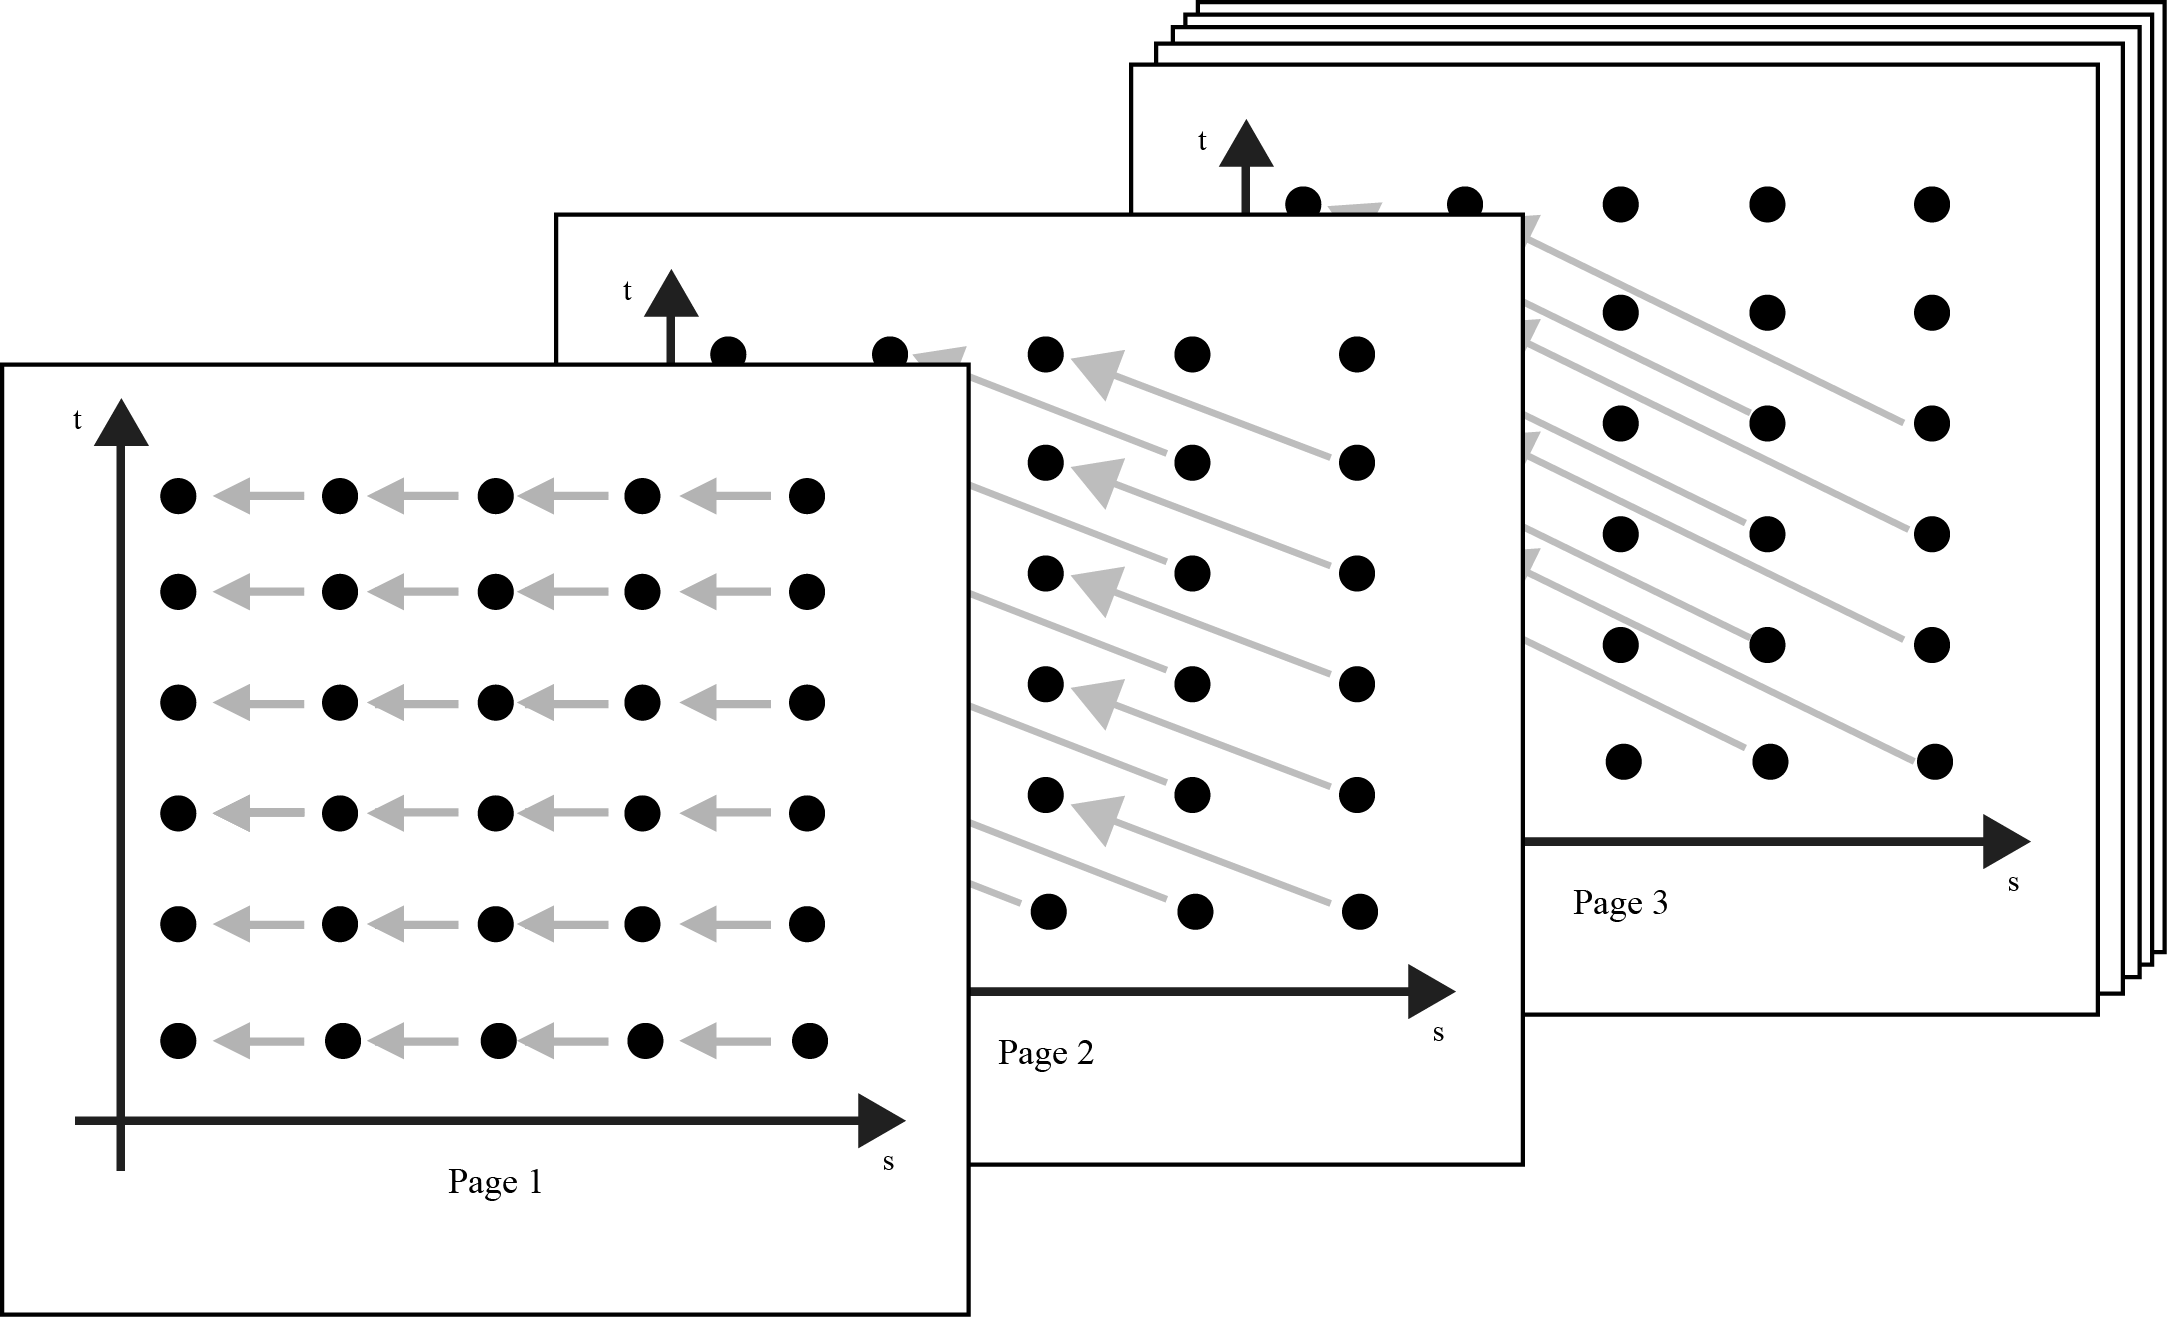
\includegraphics[width=\linewidth,height=0.5\textheight,keepaspectratio]{figures/cover.png}
  \end{center}
       \begin{minipage}{.35\linewidth}
    \begin{flushleft}
      \vspace{2em}
      {\fontsize{6pt}{2pt} \textit{Notes: These are notes live-tex'd
from a graduate course in Algebraic Curves taught by Pete Clark at the
University of Georgia in Fall 2020. As such, any errors or inaccuracies
are almost certainly my own. } } \\
    \end{flushleft}
    \end{minipage}
    \hfill
    \begin{minipage}{.65\linewidth}
    \end{minipage}
  }







\begin{document}

\date{}
\author{D. Zack Garza}
\maketitle
\begin{flushleft}
\textbf{D. Zack Garza} \\
\textit{University of Georgia} \\
\textit{dzackgarza@gmail.com} \\
{\tiny \textit{Last updated:} 2020-11-16 }
\end{flushleft}


\newpage

\tableofcontents
\newpage

\hypertarget{lecture-1}{%
\section{Lecture 1?}\label{lecture-1}}

\hypertarget{field-theory}{%
\subsection{Field Theory}\label{field-theory}}

See Chapter 11 of Field Theory notes.

\hypertarget{notion-1}{%
\subsubsection{Notion 1}\label{notion-1}}

\begin{definition}[Finitely Generated Field Extension]

A field extension \(\ell/k\) is \emph{finitely generated} if there
exists a finite set \(x_1, \cdots, x_n \in \ell\) such that
\(\ell = k(x_1, \cdots, x_n)\) and \(\ell\) is the smallest field
extension of \(k\).

Concretely, every element of \(\ell\) is a quotient of the form
\({p(x_1, \cdots, x_n) \over q(x_1, \cdots, x_n)}\) with
\(p, q\in k[x_1, \cdots, x_n]\).

\end{definition}

There are three different notions of finite generation for fields, the
above is the weakest.

\hypertarget{notion-2}{%
\subsubsection{Notion 2}\label{notion-2}}

The second is being finitely generated as an algebra:

\begin{definition}[Finitely Generated Algebras]

For \(R\subset S\) finitely generated algebras, \(S\) is finitely
generated over \(R\) if every element of \(S\) is a polynomial in
\(x_1, \cdots, x_n\), with coefficients in \(R\),
i.e.~\(S = R[x_1, \cdots, x_n]\).

\end{definition}

Note that this implies the previous definition, since anything that is a
polynomial is also a quotient of polynomials.

\hypertarget{notion-3}{%
\subsubsection{Notion 3}\label{notion-3}}

The final notion: \(\ell/k\) is finite (finite degree) if \(\ell\) is
finitely generated as a \(k\dash\)module, i.e.~a finite-dimensional
\(k\dash\)vector space.

\begin{definition}[Rational Function Field]

A \emph{rational function field} is
\(k(t_1, \cdots, t_n) \da ff \qty{ k[t_1, \cdots, t_n]}\).

\end{definition}

Note that we can make a similar definition for infinitely many
generators by taking a direct limit (here: union), and in fact every
element will only involve finitely many generators.

\begin{exercise}

\hfill

\begin{enumerate}
\def\labelenumi{\alph{enumi}.}
\item
  Show \(k(t) / k\) is finitely generated by notion (3) but not by (2).
\item
  Show that \(k[t]/k\) is (2) but not (1).
\end{enumerate}

\begin{quote}
Note \(k[t]\) is not a field.
\end{quote}

\begin{enumerate}
\def\labelenumi{\alph{enumi}.}
\setcounter{enumi}{2}
\tightlist
\item
  Show that it is not possible for a \textbf{field} extension to satisfy
  (2) but not (1).
\end{enumerate}

\begin{quote}
Hint: Zariski's lemma.
\end{quote}

\begin{enumerate}
\def\labelenumi{\alph{enumi}.}
\setcounter{enumi}{3}
\tightlist
\item
  Show that if \(\ell/k\) is finitely generated by (3) and algebraic,
  then it satisfies (1).
\end{enumerate}

\end{exercise}

\begin{theorem}[Field Theory Notes 11.19]

If \(L/K/F\) are field extensions, then \(L/F\) is finitely generated
\(\iff\) \(K/F\) and \(L/K\) are finitely generated.

\end{theorem}

\begin{quote}
See Artin-Tate Lemma, this doesn't necessarily hold for general rings.
\end{quote}

\begin{definition}[Algebraically Independent]

For \(\ell/k\), a subset \(\ts{x_i}\subset \ell\) is \emph{algebraically
independent} over \(k\) if no finite subset satisfies a nonzero
polynomial with \(k\) coefficients.

In this case, \(k[\ts{x_i}] / k\) is \emph{purely transcendental} as a
rational function field.

\end{definition}

\begin{theorem}[?]

For \(\ell/k\) a field extension,

\begin{enumerate}
\def\labelenumi{\alph{enumi}.}
\item
  There exists a subset \(\ts{x_i}\subset \ell\) algebraically
  independent over \(k\) such that \(\ell/k(\ts{x_i})\) is algebraic.
\item
  If \(\ts{y_t}\) is another set of algebraically independent elements
  such that \(\ell/k(\ts{y_t})\) is algebraic, then
  \(\abs{\ts{x_i}} = \abs{\ts{y_t}}\).
\end{enumerate}

\end{theorem}

Thus every field extension is algebraic over a purely transcendental
extension. A subset as above is called a \emph{transcendence basis}, and
every 2 such bases have the same cardinality.

We have a notion of generation (similar to ``spanning''), independence,
and bases, so there are analogies to linear algebra (e.g.~every vector
space has a basis, any two have the same cardinality). There is a common
generalization: matroids.

\begin{definition}[Transcendence Degree]

The \emph{transcendence degree} of \(\ell/k\) is the cardinality of any
transcendence basis.

\begin{quote}
Analogy: dimension in linear algebra.
\end{quote}

\end{definition}

\begin{theorem}[Transcendence Degree is Additive in Towers]

If \(L/K/F\) are fields then
\(\trdeg(L/F) = \trdeg(K/F) + \trdeg(L/K)\).

\end{theorem}

\begin{theorem}[Bounds on Transcendence Degree]

Let \(K/k\) be finitely degenerated, so \(K = k(x_1, \cdots, x_n)\).
Then \(\trdeg(K/k) \leq n\), with equality iff \(K/k\) is purely
transcendental.

\end{theorem}

\begin{proof}

Suppose \(K\) is monogenic, i.e.~generated by one element. Then
\(\trdeg(F(x)/F) = \indic{x/F\text{ is transcendental}}\).

So the degree increases when a transcendental element is added, and
doesn't change when \(x\) is algebraic.

By additivity in towers, we take
\(k \injects k(x_1) \injects k(x_1, x_2) \injects \cdots \injects k(x_1, \cdots, x)n) = K\)
to obtain a chain of length \(n\). The transcendence degree is thus the
number of indices \(i\) such that \(x_i\) is transcendental over
\(k(x_1, \cdots, x_{i-1})\).

\begin{quote}
Similar to checking if a vector is in the span of a collection of
previous vectors.
\end{quote}

\end{proof}

\begin{definition}[Function Fields]

For \(d\in\ZZ^{\geq 0}\), an extension \(K/k\) is \emph{a function field
in \(d\) variables} (i.e.~of dimension \(d\)) if \(K/k\) is finitely
generated of transcendence degree \(d\).

\end{definition}

The study of such fields is birational geometry over the ground field
\(k\). \(k=\CC\) is of modern interest, things get more difficult in
other fields.

The case of \(d=1\) is much easier: the function field will itself be
the geometric object and everything will built from that.

Main tool: valuation theory, which will correspond to points on the
curve.

\hypertarget{case-study-the-luroth-problem.}{%
\subsection{Case Study: The Luroth
Problem.}\label{case-study-the-luroth-problem.}}

For which fields \(k\) and \(d\in \ZZ^{\geq 0}\) is it true that if
\(k \subset \ell \subset k(t_1, \cdots, t_d)\) with
\(k(t_1 ,\cdots, t_d)/\ell\) finite then \(\ell\) is purely
transcendental?

\begin{theorem}[Luroth]

True for \(d=1\): For any \(k\subset \ell \subset k(t)\),
\(\ell = k(x)\).

\end{theorem}

\begin{theorem}[Castelnuovo]

Also true for \(d=2, k=\CC\).

\end{theorem}

\begin{theorem}[Zariski]

No if \(d= 2\), \(k=\bar k\), and \(k\) is positive characteristic. Also
no if \(d=2, k\neq \bar k\) in characteristic zero.

\end{theorem}

\begin{theorem}[Clemens-Griffiths]

No if \(d\geq 3\) and \(k= \CC\).

\end{theorem}

\begin{quote}
Unirational need not imply rational for varieties.
\end{quote}

\begin{exercise}

Let \(k\) be a field, \(G\) a finite group with \(G\injects S_n\) the
Cayley embedding. Then \(S_n\) acts by permutation of variables on
\(k(t_1, \cdots, t_n)\), thus so does \(G\). Set
\(\ell \da k(t_1, \cdots, t_n)^G\) the fixed field, then by Artin's
observation in Galois theory: if you have a finite field acting
effectively by automorphisms on a field then taking the fixed field
yields a galois extension with automorphism group \(G\).

So \(\aut(k(t_1, \cdots, t_n)/ \ell) = G\).A

\begin{enumerate}
\def\labelenumi{\alph{enumi}.}
\tightlist
\item
  Suppose \(k=\QQ\), and show that an affirmative answer to the Luroth
  problem implies an affirmative answer to the inverse galois problem
  for \(\QQ\).
\end{enumerate}

\begin{quote}
Hint: works for any field for which Hilbert's Irreducibility Theorem
holds.
\end{quote}

\begin{enumerate}
\def\labelenumi{\alph{enumi}.}
\setcounter{enumi}{1}
\item
  \(\ell /\QQ\) need not be a rational function field, explore the
  literature on this: first example due to Swan with \(\abs{G} = 47\).
\item
  Can still give many positive examples using the Shepherd-Todd Theorem.
\end{enumerate}

\end{exercise}

\todo[inline]{What's a global field?}

\hypertarget{onto-business}{%
\subsection{Onto Business}\label{onto-business}}

\begin{definition}[?]

For \(K/k\) a field extension, set \(\kappa(K)\) to be the algebraic
closure of \(k\) in \(K\), i.e.~special case of \emph{integral closure}.
If \(K/k\) is finitely generated, then \(\kappa(K)/k\) is finite degree.

Here \(\kappa(k)\) is called the \emph{field of constants}, and \(K\) is
also a function field over \(\kappa(k)\).

\end{definition}

In practice, we don't want \(\kappa(k)\) to be a proper extension of
\(k\).

If this isn't the case, we replace considering \(K/k\) by
\(K/\kappa(k)\). If \(K/k\) is finitely generated, then

\begin{center}
\begin{tikzcd}
k \arrow[rr, "\text{finite}", hook] &  & \kappa(k) \arrow[rr, "\text{finitely generated}", hook] &  & K
\end{tikzcd}
\end{center}

Where we use the fact that from above, \(\kappa(k)/k\) is finitely
generated and algebraic and thus finite, and by a previous theorem, if
\(K/k\) is transcendental then \(K/\kappa(k)\) is as well, and thus
finitely generated. Thus if you have a function field over \(k\), you
can replace \(k\) by \(\kappa(k)\) and regard \(K\) as a function field
over \(\kappa(k)\) instead.

\hypertarget{lecture-1-a-review}{%
\subsection{Lecture 1, A Review}\label{lecture-1-a-review}}

Review of lecture one:

\begin{theorem}[Finitely Generated in Towers]

See video

\end{theorem}

\begin{itemize}
\tightlist
\item
  Transcendence bases
\item
  Lüroth problem
\end{itemize}

\hypertarget{lecture-2}{%
\section{Lecture 2?}\label{lecture-2}}

For \(K/k\) a one variable function field, if we want a curve \(C/k\),
what are the points? We'll use \emph{valuations}, see NT 2.1.

See also completions, residue fields.

If \(R \subset K\) a field, \(R\) is a \emph{valuation ring} of \(K\) if
for all \(x\in K\units\), at least one of \(x, x^{-1} \in R\).

\begin{example}

The valuation rings of \(\QQ\) are
\(\ZZ_{(p)}\da \ZZ[\ts{{1\over \ell} \st \ell\neq p}]\) for all primes
\(p\).

\end{example}

See also Krull valuation, takes values in some totally ordered
commutative group.

\begin{exercise}

Show that a valuation ring is a local ring, i.e.~it has a unique maximal
ideal.

\end{exercise}

\begin{example}

Where does the log come from?

There is a \(p\dash\)adic valuation:
\begin{align*}  
v: \QQ &\to \ZZ_{(p)} \\
{a\over b} = p^n {u \over v} &\mapsto n
.\end{align*}

Then we recover
\begin{align*}  
\ZZ_{(p)} = \ts {x\in \QQ\units \st v_p(x) \geq 0} \union \ts{0} \\
\mfm_{(p)} = \ts {x\in \QQ\units \st v_p(x) > 0} \union \ts{0} \\
.\end{align*}

There is a \(p\dash\)adic norm
\begin{align*}  
\abs{\wait}_p: \QQ &\to \RR \\
0 & \mapsto 0 \\
x &\mapsto p^{-n} = p^{-v_p(x)}
.\end{align*}

Then we get an ultrametric function, a non-archimedean function
\begin{align*}  
d_p: \QQ^2 \to \RR \\
(x, y) &\mapsto \abs{x- y}_p
.\end{align*}

We then recover \(v_p(x) = -\log_p \abs{x}_p\).

See NT 1 notes.

\end{example}

For \(A\subset K\) a subring of a field, we'll be interested in the
place
\(\tilde \Sigma = \ts{\text{Valuation rings } R_v \text{ of } K} \st A \subset R_v \subsetneq K\).
Thus the valuation takes non-negative values on all elements of \(K\).
Can equip this with a topology (the ``Zariski'' topology, not the usual
one). This is always quasicompact, and called the \emph{Zariski-Riemann
space}. Can determine a sheaf of rings to make this a locally ringed
space.

We can define an equivalence of valuations and define the set of
\emph{places}
\begin{align*}  
\Sigma(K/k) \da \ts{\text{Nontrivial valuations } v\in K \st v(x) \geq 0\, \forall x\in k\units}
,\end{align*} which will be the points on the curve. Here the Zariski
topology will be the cofinite topology (which is not Hausdorff).
Scheme-theoretically, this is exactly the set of closed points on the
curve.

\begin{definition}[?]

Generic point: closure is entire space.

\end{definition}

\begin{quote}
Note we will have unique models for curves, but this won't be the case
for surfaces: blowing up a point will yield a birational but
inequivalent surface.
\end{quote}

From this we can also define \emph{divisor group} as the free
\(\ZZ\dash\)module on \(\Sigma(K/k)\), which comes with a degree map
\begin{align*}  
\deg: \Div(K) \to \ZZ
\end{align*} which need not be surjective.

We can consider principle divisors with the map
\begin{align*}  
K\units &\to \Div(K) \\
f &\mapsto (f)
.\end{align*}

We can define the class group as divisors modulo principle divisors
\(\cl(K) = \Div(K) / \im(K\units)\) and the Riemann-Roch space
\(\mathcal{L}(D)\). The Riemann-Roch theorem will then be a statement
about \(\dim \mathcal{L}(D)\).

\hypertarget{lecture-3}{%
\section{Lecture 3}\label{lecture-3}}

\hypertarget{base-extension}{%
\subsection{Base Extension}\label{base-extension}}

Given some object \(A/k\) and \(k\injects \ell\) is a field extension,
we would like some extended object \(A/\ell\).

\begin{example}

An \emph{affine variety} \(V/k\) is given by finitely many polynomials
in \(p_i \in k[t_1, \cdots, t_n]\), and base extension comes from the
map \(k[t_1, \cdots, t_n] \injects \ell[t_1, \cdots, t_n]\).

More algebraically, we have the affine coordinate ring over \(k\) given
by \(k[V] = k[t_1,\cdots, t_n]/\gens{p_i}\), the ring of polynomial
functions on the zero locus corresponding to this variety. We can
similarly replace \(k\) be \(\ell\) in this definition. Here we can
observe that \(\ell[V] \cong k[V] \tensor_k \ell\).

\end{example}

In general we have a map
\begin{align*}  
\wait \tensor_k \ell & \\
\ts{k\dash\text{vector spaces}} &\to \ts{\ell\dash\text{vector spaces}} \\
\ts{k\dash\text{algebras}} &\to\ts{\ell\dash\text{algebras}}
.\end{align*}

Note that this will be an exact functor on the category
\(k\dash\text{Vect}\), i.e.~\(\ell\) is a flat module. Here everything
is free, and free \(\implies\) flat, so things work out nicely.

What about for function fields?

Since \(k\) is a \(k\dash\)algebra, we can consider \(k\tensor_k \ell\),
however this need not be a field.

\begin{quote}
Note: tensor products of fields come up very often, but don't seem to be
explicitly covered in classes! We'll broach this subject here.
\end{quote}

\begin{exercise}

If \(\ell/k\) is algebraic and \(\ell\tensor_k \ell\) is a domain, the
\(\ell = k\).

\begin{quote}
I.e. this is rarely a domain. Hint: start with the monogenic case, and
also reduce to the case where the extension is not just algebraic but
finite.
\end{quote}

\end{exercise}

Tensor products of field extensions are still interesting: if \(\ell/k\)
is finite, it is galois \(\iff\)
\(\ell \tensor_k \ell \cong \ell^{[\ell: k]}\). So its dimension as an
\(\ell\dash\)algebra is equal to the degree of \(\ell/k\), so it splits
as a product of copies of \(\ell\).

\begin{remark}

We'd like the tensor product of a field to be a field, or at least a
domain where we can take the fraction field and get a field. This hints
that we should not be tensoring algebraic extensions, but rather
transcendental ones.

\end{remark}

\begin{exercise}

For \(\ell/k\) a field extension,

\begin{enumerate}
\def\labelenumi{\alph{enumi}.}
\item
  Show \(k(t) \tensor_k \ell\) is a domain with fraction field
  \(\ell(t)\).
\item
  Show it is a field \(\iff\) \(\ell/k\) is algebraic.
\end{enumerate}

\end{exercise}

\begin{proposition}[FT 12.7, 12.8]

Let \(k_1, k_2 / k\) are field extensions, and suppose
\(k_1 \tensor_k k_2\) is a domain. Then this is a field \(\iff\) at
least one of \(k_1/k\) or \(k_2/k\) is algebraic.

\end{proposition}

\begin{quote}
Reminder: for \(\ell/k\) and \(\alpha\in \ell\) algebraic over \(k\),
then \(k(\alpha) = k[\alpha]\).
\end{quote}

So we'll concentrate on when \(K \tensor_k \ell\) is a domain. What's
the condition on a function field \(K/k\) that guarantees this,
i.e.~when extending scalars from \(k\) to \(\ell\) still yields a
domain? If this remains a domain, we'll take the fraction field and call
it the \emph{base change}.

\begin{exercise}

If \(K/k\) is finitely generated (i.e.~a function field) and
\(K\tensor_k \ell\) is a domain, then \(ff(K\tensor_k \ell)/\ell\) is
finitely generated.

\begin{quote}
The point: if taking a function field and extending scalars still
results in a domain, we'll call the result a function field as well.
\end{quote}

\end{exercise}

Most of all, we want to base change to the algebraic closure. We'll have
issues if the constant field is not just \(k\) itself:

\begin{lemma}

If \(K\tensor_k \bar k\) is a domain, then the constant field
\(\kappa(k) = k\).

\end{lemma}

\begin{proof}

Use the fact that \(\wait \tensor_k V\) is exact. We then get an
injection

\begin{center}
\begin{tikzcd}
\kappa(k) \tensor_k \kappa(k) \ar[rr, hookrightarrow]\ar[rd, hookrightarrow] & &
K \tensor_k \bar k \\
& \kappa(k) \tensor_k \bar k\ar[ru, hookrightarrow] & 
\end{tikzcd} 
\end{center}

Here we use the injections \(\kappa(k) \injects \bar k\) and
\(\kappa(k) \injects K\).

We now have an injection of \(k\dash\)algebras, and subrings of domains
are domains. So apply the first exercise: the only way this can happen
is if \(\kappa(k) = k\).

\end{proof}

\begin{exercise}

The simplest possible case: describe \(\CC(t) \tensor_\RR \CC\),
tensored as \(\RR\dash\)algebras.

\begin{quote}
Won't be a domain by the lemma, some \(\CC(t)\dash\)algebra of dimension
2.
\end{quote}

\end{exercise}

In order to have a good base change for our function fields, we want to
constant extension to be trivial, i.e.~\(\kappa(k) = k\). This requires
that the ground field be algebraically closed.

In this case, you might expect that extending scalars to the algebraic
closure would yield a field again. This is true in characteristic zero,
but false in positive characteristic.

A more precise question: if \(\kappa(k) = k\), must
\(K\tensor_K \bar k\) be a field? If that's true and we're in positive
characteristic, recalling the for an algebraic extension this being a
field is equivalent to it being a domain. But if that's a domain, the
tensor product of every algebraic extension must be a domain, which is
why this is an important case.

If so, then \(K\tensor_k k^{1\over p}\) is a field, where
\(k^{1\over p} \da k(\ts{x^{1\over p} \st x\in k })\) is obtained by
adjoining all \(p\)th roots of all elements. This is a purely
inseparable extension. The latter condition (this tensor product being a
field) is one of several equivalent conditions for a field to be
separable.

\begin{quote}
Note that frobenius maps \(k^{1\over p} \surjects k\), so this is sort
of like inverting this map.
\end{quote}

Remember that \(K/k\) is transcendental, and there is an extended notion
of separability for non-algebraic extensions. Another equivalent
condition is that every finitely generated subextension is separably
generated, i.e.~it admits a transcendence basis \(\ts{x_i}\) such that
\(k\injects k(\ts{x_i}) \injects F\) where \(F/k(\ts{x_i})\) is
algebraic and separable. Such a transcendence basis is called a
\emph{separating transcendence basis}. Since we're only looking at
finitely generated extensions, we wont' have to worry much about the
difference between separable and separably generated.

What's the point? There's an extra technical condition to ensure the
base change is a field: the function field being separable over the
ground field.

Is this necessarily the case if \(\kappa(k) = k\)? No, for a technical
reason:

\begin{warning}

This is pretty technical, yo.

\end{warning}

\begin{example}

\label{technical_example} Set \(k = \FF_p(a, b)\) a rational function
field in two variables sa the ground field. Set
\begin{align*}  
A \da k[x, y]/ \gens{ax^p + b-y^b}
.\end{align*} Then \(A\) is a domain, so set \(k = ff(A)\).

Claim: \(\kappa(k) = k\), so \(k\) is algebraically closed in this
extension, but \(K/k\) is \emph{not} separable. How to show: extending
scalars to \(k^{1\over p}\) does not yield a domain.

Let \(\alpha, \beta \in \bar k\) such that
\(\alpha^p = a, \beta^b = b\), so
\begin{align*}  
ax^p + b-y^b = (\alpha x + \beta - y)^p
,\end{align*} which implies \(K \tensor_k k^{1\over p}\) is not a
domain: \(k[x, y]\) is a UFD, so the quotient of a polynomial is a
domain iff the polynomial is irreducible. However, the \(p\)th power map
is a homomorphism, and this exhibits the image of the defining
polynomial as something non-irreducible.

\end{example}

Note that \(f(x, y) = ax^p + b - y^p\) is the curve in this situation.
The one variable function field is defined by quotienting out a function
in two variables and taking the function field. Every 1-variable
function field can be obtained in this way. Therefore this polynomial is
irreducible, but becomes reducible over the algebraic closure. So we'd
like the polynomial to be irreducible over both.

\begin{remark}

This is pretty technical, but we won't have to worry if
\(k = k^{1\over p}\). Equivalently, frobenius is surjective on \(k\),
i.e.~\(k\) is a perfect field.

If \(k\) is not perfect, it can happen (famous paper of Tate) making an
inseparable base extension can decrease the genus of the curve.

\end{remark}

Reminder: the perfect fields:

\begin{itemize}
\tightlist
\item
  Anything characteristic zero, every reducible polynomial is separable.
\item
  Any algebraically closed field
\item
  Finite fields (frobenius is always injective)
\end{itemize}

Imperfect fields include:

\begin{itemize}
\tightlist
\item
  Function fields in characteristic \(p\)
\item
  Complete discretely valued fields \(k((t))\) in characteristic \(p\)
\end{itemize}

\todo[inline]{Look up uniformizing elements and valuations.}

\begin{theorem}[FT 12.20]

For field extensions \(K/k\), TFAE

\begin{enumerate}
\def\labelenumi{\arabic{enumi}.}
\item
  \(\kappa(k) = k\) and \(K/k\) is separable
\item
  \(K\tensor_k \bar k\) is a domain, or equivalently a field
\item
  For all field extensions \(\ell/k\), \(K\tensor_k \ell\) is a domain.
\end{enumerate}

\begin{quote}
Allows making not just an algebraic base change, but a totally arbitrary
one.
\end{quote}

\end{theorem}

A field extension satisfying these conditions is called
\textbf{regular}.

\begin{quote}
Regular corresponds to nonsingularity in this neck of the woods.
\end{quote}

\begin{remark}

The implication \(2\implies 3\) is the interesting one. To prove it,
reduces to showing that if \(k= \bar k\) and \(R_i\) are domains that
are finitely generated as \(k\dash\)algebras, then \(R_1 \tensor_k R_2\)
is also a domain.

This doesn't always happen,
e.g.~\(\QQ(\sqrt{2}) \tensor_\QQ \QQ(\sqrt{2})\) is not a domain. Really
need algebraically closed.

This is a result in affine algebraic geometry. An algebra that is a
domain and finitely generated over a field is an \emph{affine algebraic
variety}, more precisely it is integral. The tensor product on the
coordinate ring side corresponds to taking the product of varieties.

Thus the fact here is that a product of integral varieties remains
integral, as long as you're over an algebraically closed field. Proof
uses Hilbert's Nullstellensatz.

\end{remark}

\begin{exercise}

\hfill

\begin{enumerate}
\def\labelenumi{\alph{enumi}.}
\tightlist
\item
  Show that \(k(t) / k\) is regular.
\end{enumerate}

\begin{quote}
I.e. \(k(t)\tensor_k \bar k\) is a domain.
\end{quote}

\begin{enumerate}
\def\labelenumi{\alph{enumi}.}
\setcounter{enumi}{1}
\item
  Show every purely transcendental extension is regular.
\item
  Show that for a field \(k\), every extension is regular \(\iff\)
  \(k = \bar k\).
\item
  Show \(K/k\) is regular \(\iff\) every finitely generated subextension
  is regular.
\end{enumerate}

\end{exercise}

\hypertarget{example-of-a-non-regular-family-of-function-fields}{%
\subsection{Example of a Non-Regular Family of Function
Fields}\label{example-of-a-non-regular-family-of-function-fields}}

Choose an elliptic curve \(E/\QQ(t)\) with \(j\dash\)invariant \(t\).
For \(N\in \ZZ^{+}\), define \(\tilde K_N \da \QQ(t)(E[N])\) the
\(N\dash\)torsion field of \(E\).

Then \(\tilde K_N/\QQ(t)\) is a finite galois extension with galois
group isomorphic to the image of the modular galois representation
\begin{align*}  
\rho_N: g(\QQ(t)) \to \GL(2, \ZZ/N\ZZ) \mod N
.\end{align*}

\begin{quote}
See Cornell-Silverman-Stevens covering the proof of FLT, modular curves
from the function field perspective.
\end{quote}

\begin{proposition}[Some Facts]

\(\rho_N\) is surjective, and
\begin{align*}  
\Aut(\tilde K_N / \QQ(t))  \cong \GL(2, \ZZ/N\ZZ)
.\end{align*}

\(\det \rho_N = \chi_N \mod N\), the cyclotomic character, and therefore
\(\chi_N\) restricted to \(g(\tilde K_N)\) is trivial, so
\(\tilde K_N \supset \QQ(\zeta_N)\). For \(N\geq 3\),
\(\QQ(\zeta_N) \supsetneq \QQ\), so \(\tilde K_N / \QQ(t)\) is a
non-regular function field.

\end{proposition}

Actually \(\tilde K_N\) depends on the choice of \(E\): difference
choices of nonisomorphic curves with the same \(j\dash\)invariant differ
by a quadratic twist and the \(\rho_N\) differ by a quadratic character
on \(g(\QQ(t))\). Importantly, this changes the kernel, and thus the
field.

To fix this, we look at the \emph{reduced galois representation}, the
following composition:
\begin{align*}  
\bar \rho_N: g(\QQ(t)) \to \GL(2, \ZZ/N\ZZ) \surjects \GL(2, \ZZ/N\ZZ)/\ts{\pm I}
.\end{align*}

We obtain a field theory diagram

\begin{center}
\begin{tikzcd}
\ar[dd, bend right, "{\GL(2, \ZZ/N\ZZ)}"'] \bar K_N \ar[d, bend left, "\ts{\pm I}"] &\\
K_N \ar[d, bend left, "{\GL(2, \ZZ/N\ZZ)/\ts{\pm I}}"] &\\
\QQ(t)&
\end{tikzcd}
\end{center}

So if you just take the field fixed by \(\pm I\), you get \(K_N\). In
this case, the reduced galois representation depends only on the
\(j\dash\)invariant, and not on the model chosen. So the function field
\(K_N/\QQ(t)\) is the ``canonical'' choice.

Question: Does this make \(K_N/\QQ(t)\) regular?

Answer: No, \(\rho_N(g(K_N)) = \ts{\pm I}\) and \(\det(\pm I) = 1\), so
we still have \(K_N \supset \QQ(\zeta_N)\).

In this course, we'll identify algebraic curves over \(k\) and
one-variable function fields \(K/k\). The function field \(K_N\)
corresponds to an algebraic curve \(X(N)/\QQ\) that is ``nicer'' over
\(\QQ(\zeta_N)\). In fact, see Rohrlich: \(\kappa(K_N) = \QQ(\zeta_N)\).

Our curves will have points (equal to valuations) which will have
degrees. If the constant subfield is not just \(k\), this prevents
degree 1 points on the curve.

By Galois theory, for every subgroup
\(H \subseteq \GL(2, \ZZ/N\ZZ) / \ts{\pm I}\), we'll get a function
field \(\QQ(H) \da H_N^H\). In this case, \(\QQ(H)/\QQ\) is regular
\(\iff\) \(\det(H) = (\ZZ/N\ZZ)\units\).

Later we'll understand the residues at points as the residue fields of
some DVRs, then the residue field will always contain the field of
constants.

\hypertarget{lecture-4}{%
\section{Lecture 4}\label{lecture-4}}

Last of preliminaries. Upcoming: one-variable function fields and their
valuation rings.

\hypertarget{polynomials-defining-regular-function-fields}{%
\subsection{Polynomials Defining Regular Function
Fields}\label{polynomials-defining-regular-function-fields}}

Where's the curve: \(f(x, y) = 0\).

\begin{exercise}

Let \(R_1, R_2\) be \(k\dash\)algebras that are also domains with
fraction fields \(K_i\). Show \(R_1 \tensor_k R_2\) is a domain \(\iff\)
\(K_1 \tensor_k K_2\) is a domain.

\begin{quote}
Denominator-clearing argument.
\end{quote}

\end{exercise}

\begin{definition}[Geometrically Irreducible]

A polynomial of positive degree \(f\in k[t_1, \cdots, t_n]\) is
\emph{geometrically irreducible} if \(f\in \bar k[t_1, \cdots, t_n]\) is
irreducible as a polynomial.

\end{definition}

If \(n=1\) then \(f\) is geometrically irreducible \(\iff\) it's linear,
i.e.~of degree 1.

Let \(f\) be irreducible, then since polynomial rings are UFDs then
\(\gens{f}\) is a prime ideal (irreducibles generate principal ideals)
and \(k[t_1, \cdots, t_n]/\gens{f}\) is a domain. Let \(K_f\) be the
fraction field.

\begin{exercise}

Easy:

\begin{enumerate}
\def\labelenumi{\alph{enumi}.}
\item
  Above for \(1\leq i \leq n\) let \(x_i\) be the image of \(t_i\) in
  \(K_f\). Show that \(K_f = k(x_1, \cdots, x_n)\).
\item
  Show that if \(K/k\) is generated by \(x_1, \cdots, x_n\), then it is
  the fraction field of \(k[t_1, \cdots, t_n] /\mfp\) for some prime
  ideal \(\mfp\) (equivalently, a height 1 ideal).
\end{enumerate}

\end{exercise}

\begin{proposition}[?]

Suppose that \(f\) is geometrically irreducible.

\begin{enumerate}
\def\labelenumi{\alph{enumi}.}
\item
  The function field \(K/k\) is regular.
\item
  For all \(\ell/k\), \(f\in \ell[t_1, \cdots, t_n]\) is irreducible.
\end{enumerate}

\begin{quote}
In this case we say \(f\) is \emph{absolutely irreducible} as a synonym
for geometrically irreducible.
\end{quote}

\end{proposition}

\begin{proof}

By definition of geometric irreducibility,
\(\bar k[t_1, \cdots, t_n]/\gens{f} = k[t_1, \cdots, t_n]/\gens{f} \tensor_k \bar k\)
is a domain. The exercise shows that \(K_f \tensor_k k\) is a domain, so
\(K_f\) is regular.

It follows that for all \(\ell/k\), \(K_f \tensor_k \ell\) is a domain,
so \(\ell[t_1, \cdots, t_n]/\gens{f}\) is a domain.

\end{proof}

Moral: geometrically irreducible polynomials are good sources of regular
function fields.

\begin{exercise}

Let \(k\) be a field, \(d\in \ZZ^+\) such that \(4\notdivides d\) and
\(p(x) \in k[x]\) be positive degree. Factor
\(p(x) = \prod_{i=1}^r (x-a_i)^{\ell_i}\) in \(\bar k[x]\).

\begin{enumerate}
\def\labelenumi{\alph{enumi}.}
\tightlist
\item
  Suppose that for some \(i\), \(d\notdivides \ell_i\). Show that
  \(f(x, y) \da y^d - p(x) \in k[x, y]\) is geometrically irreducible.
  Conclude that \(K_f \da ff\qty{k[x, y] / \gens{y^d - p(x)}}\) is a
  regular one-variable function field over \(k\), and thus elliptic
  curves yield regular function fields.
\end{enumerate}

\begin{quote}
Referred to as \emph{hyperelliptic} or \emph{superelliptic} function
fields. Hint: use FT 9.21 or Lang's Algebra.
\end{quote}

\begin{enumerate}
\def\labelenumi{\alph{enumi}.}
\setcounter{enumi}{1}
\tightlist
\item
  What happens when \(4\divides d\)?
\end{enumerate}

\end{exercise}

\begin{exercise}[Nice, Recommended]

Assume \(k\) is a field, if necessary assuming \(\ch(k) \neq 2\).

\begin{enumerate}
\def\labelenumi{\alph{enumi}.}
\item
  Let \(f(x, y) = x^2 - y^2 -1\) and show \(K_f\) is is rational:
  \(K_f = k(z)\).
\item
  Let \(f(x, y) = x^2 + y^2 - 1\). Show that \(K_f\) is again rational.
\item
  Let \(k = \CC\) and \(f(x, y) = x^2 + y^2 + 1\), \(K_f\) is rational.
\item
  Let \(k= \RR\). For \(f(x ,y) = x^2 + y^2 + 1\), is \(K_f\) rational?
\end{enumerate}

\begin{quote}
Example of a non-rational genus zero function field.
\end{quote}

\end{exercise}

Question (converse): Can we always construct regular function fields
using geometrically irreducible polynomials?

Answer: In several variables, no, since not every variety is birational
to a hypersurface.

In one variable, yes:

\begin{theorem}[Regular Function Fields in One Variable are Geometrically Irreducible]

Let \(K/k\) be a one variable function fields (finitely generated,
transcendence degree one). Then

\begin{enumerate}
\def\labelenumi{\alph{enumi}.}
\item
  If \(K/k\) is separable, then \(K = k(x, y)\) for some \(x, y\in K\).
\item
  If \(K/k\) is regular (separable + constant subfield is \(k\), so
  stronger) then \(K \cong K_f\) for a geometrically irreducible
  \(f\in k[x ,y]\).
\end{enumerate}

\end{theorem}

\begin{proof}

Recall separable implies there exists a separating transcendence basis.

Proof of (a):

This means there exists a primitive element \(x\in K\) such that
\(K/k(x)\) is finite and separable. By the Primitive Element Corollary
(FT 7.2), there exist a \(y\in K\) such that \(K = k(x, y)\).

Proof of (b):

Omitted for now, slightly technical.

\end{proof}

Importance of last result: a regular function field on one variable
corresponds to a nice geometrically irreducible polynomial \(f\).

\begin{quote}
Note: the plane curve module may not be smooth, and in fact usually is
not possible. I.e. \(k[x ,y]/\gens{f}\) is a one-dimensional noetherian
domain, which need not be integrally closed.
\end{quote}

Question: Can every one variable function field be 2-generated?

Answer: Yes, as long as the ground field is perfect. In positive
characteristic, the suspicion is no: there exists finite inseparable
extensions \(\ell/k\) that need arbitrarily many generators.

However, what if \(K/k\) has constant field \(k\) but is not separable?
Riemann-Roch may have something to say about this.

\begin{example}

\hyperref[technical_example]{Example from earlier lecture:}

\(ax^p + b - y^b\)

\end{example}

Moral: look for examples of nice function fields by taking irreducible
polynomials in two variables. This will define a one-variable function
field. If the polynomial is geometrical reducible, this produces regular
function fields.

Next: One variable function fields and their valuations.

\hypertarget{lecture-13}{%
\section{Lecture 13}\label{lecture-13}}

Recall that we previously looked at the regular function fields: we took
a function field in one variable and considered the class of function
fields for which we could take any extension of the constant field that
we wanted. As long as the ground field is perfect, being regular is
equivalent to the constant subfield being \(k\) itself. However, we
haven't done anything with them yet!

If you take an algebraic closure of the finite ground field \(\FF_q\),
there is a unique subextension of degree \(r\) for every \(r\), so we
call that \(\FF_{q^r}\). The extension \(\FF_{q^r}/\FF_q\) is cyclic
galois, with a geometric Frobenius \(x\to x^q\). Note that \(\FF_{q^r}\)
is the fixed field of \(F^r\), the \(r\)th power of the Frobenius map.
We set \(K_r \da K \FF_{q^r}\), which is a regular function field over
\(\FF_{q^r}\). Note that we could view this as a function field just
over \(\FF_q\), but it would not be regular. Then \(K_r/K\) is a degree
\(r\) arithmetic extension of function fields.

Question: What happens to places when making this scalar extension?
I.e., how to places in \(K\) decompose in \(K_r\)?

\begin{remark}

This is related to an Algebraic Number Theory I problem: for
\(v\in \Sigma(\kfq)\) above an affine Dedekind domain \(R\) such that
\(v\in \Sigma(K/R)\), let \(S\) be the integral closure of \(K\) in
\(K_r\). Then we want to factor \(p_v S\)?
\todo[inline]{Not quite sure.}

\end{remark}

\begin{lemma}[Key lemma about how places split.]

Suppose \(d\da \deg(v)\). Then \(K_r/K\) is galois, so we have
\(efg=r\). In fact, \(c=1\), so \(f = {r\over \gcd(d, r)}\) and
\(g = \gcd(d, r)\) and each place \(w\in \Sigma(K_r / \FF_{q^r})\) has
degree \({d\over \gcd(d, r)}\).

\end{lemma}

\begin{remark}

We have the following cases:

\begin{itemize}
\item
  The extension is \emph{inert} iff \(\gcd(d, r) = 1\),
\item
  The extension \emph{splits completely} iff \(r\divides d\),
\item
  All \(w\) dividing \(v\) have degree 1 iff \(d\divides r\).
\end{itemize}

\end{remark}

The last thing we proved was that the degree zero divisor class group is
finite when we're over a finite ground field. Why is this true? Whenever
there is a divisor of degree \(n\), then the set of degree \(n\)
divisors is a coset of the degree zero divisors, all of which have the
same cardinality. We proved finiteness using the Riemann-Roch theorem,
using the fact that the set of \emph{effective} degree \(n\) divisors is
finite for all \(n\).

The next main topic will be the zeta function, which keeps track of
three equivalent packets of information: \(A_n\), the number of
effective divisors of degree \(n\), the number of places of degree \(d\)
(since an effective divisor is a linear combination of these), and
\(N_r\) the number of degree 1 points in the degree \(r\) extension,
i.e.~the number of \(\FF_{q^r}\) rational points.

\begin{lemma}[?]

Suppose \(C\in \Cl(K)\), then

\begin{itemize}
\item
  The number of effective divisors \(D \in [C]\) is given by
  \begin{align*}  
  {q^{\ell(C)} -1 \over q-1} 
  ,\end{align*} where \(\ell(C)\) is the dimension of the linear system
  associated to the divisor class \(C\), and this is the dimension of a
  projective space over \(\FF_q\).
\item
  For all \(n>2g-2\) with \(\delta \divides n\), we have
  \begin{align*}  
  A_n = h \qty{ q^{n+1-g} - 1\over q-1}
  .\end{align*}
\end{itemize}

\end{lemma}

\begin{proof}[?]

\envlist

\textbf{Proof of (a)}: The set of effective divisors linearly equivalent
to \(D\) is naturally viewed as the projectivization
\(\PP \mathcal{L}(D)\) of the one-dimensional subspaces of the linear
system of that divisor class. It is then a fact that the number of
elements in a \(d\dash\)dimensional vector space over \(\FF_q\) has
dimension precisely \(\frac{q^d-1}{q-1}\) elements. The projectivization
comes in because two different functions have the same divisor if one of
them is a constant multiple of the other. Note that the number of
elements is computed as the number of nonzero elements divided by the
number of nonzero scalars.\\

\textbf{Proof of (b)}: This will come out of the Riemann-Roch theorem.
In order to compute the number of divisors in a divisor class, you need
to know the dimension of the linear system, which is not easy in
general. However, if the divisor class has sufficiently large degree,
the Riemann-Roch theorem tells you exactly what it is. As long as
\(n > 2g-2\), there is no correction term, and the dimension of the
linear system is equal to its degree minus the genus plus one. So by
Riemann-Roch, since \(\deg(D) > 2g-2\), \(D\) is non-special and
\(\ell([D]) = n-g+1\), which yields the desired formula for \(A_n\).

\end{proof}

\begin{remark}

This is the sharpest result possible: the canonical divisor has degree
\(2g-2\) and is special, so this fails for the canonical class.

\end{remark}

Upshot: there are three piece of information:

\begin{itemize}
\item
  \(N_r\), the number of \(\FF_{q^r}\) rational points,
\item
  \(\abs{\Sigma_d(\kfq)}\) the number of closed points / places of
  degree \(d\),
\item
  \(A_n\) the number of effective divisors of degree \(n\),
\end{itemize}

and there are simple formulas relating these. Moreover, it is enough to
know only finitely many of these quantities, where the number depends on
\(g\).

\hypertarget{hasse-weil-zeta-functions}{%
\subsection{Hasse-Weil Zeta Functions}\label{hasse-weil-zeta-functions}}

There is a general theory that will unify

\begin{itemize}
\item
  The Riemann zeta function, thought of as the zeta function of \(\ZZ\),
\item
  The Dedekind zeta function, attached to the ring of integers over a
  number field,
\item
  The Hasse-Weil zeta function of a one variable function field over a
  finite field,
\end{itemize}

all of which will be special cases of a \emph{Serre zeta function} which
can be attached to a finite type scheme over \(\ZZ\).

Note that we aren't specifically discussing schemes in this course, but
you don't need to know much about what a scheme is to define the
Hasse-Weil zeta function. Just note that an affine finite-type
\(\ZZ\dash\)scheme corresponds to a finitely generated
\(\ZZ\dash\)algebra, and a general finite-type \(\ZZ\dash\)scheme will
be covered by finitely many affine ones, the zeta function will be
determined by these finitely many \(\ZZ\dash\)algebras and some kind of
inclusion-exclusion principle (since the scheme is a not necessarily
disjoint union of affine schemes).

Recall that \(A_n = A_n(K)\) is the number of effective divisors of
degree \(n\), which we've proved is finite. We have a formula when
\(n> 2g-2\), namely
\begin{align*}  
Z(t) = \sum_{n=0}^\infty A_n t^n = \sum_{D\in \Div^+(K)} t^{\deg(D)} \in \ZZ[[t]]
,\end{align*} where \(\Div^+\) are the effective divisors and we've
collected terms based on their degree. This is analogous to the Dedekind
zeta function of a number field \(K\), a formal Dirichlet series which
is given by
\begin{align*}  
\zeta_K(s) = \sum_{I \in \mathcal{I}\qty{\ZZ_K^\bullet}} \abs{ \ZZ_K / I}^{-s}
.\end{align*} where the sum is now over all of the nonzero ideals of the
ring of integers, where we measure the size using the \emph{norm},
i.e.~the size of the residue field. There's an analogy between integral
ideals (vs fractional ideals) and effective divisors. We could get an
Euler product decomposition for the Dedekind zeta function by only
considering prime ideals, since in a Dedekind domain all ideals factor
uniquely into prime ideals. In fact, any nonzero ideal is a linear
combination of prime ideals. Similarly, the effective divisors are
linear combinations of effective divisors, so an Euler product expansion
is possible here too. If we take a prime ideal, since we're in a
discrete valuation ring, we can consider the local ring at that point.
We can take the residue field, which in general won't be finite, but
will be a finite extension. So a reasonable measure of the size of a
prime divisor would be the dimension of its residue field as a vector
space over \(K\).

Note that if we wanted to make these look even more similar to each
other, we could define \(a_n\) (depending on \(\ZZ_K\)) as
\begin{align*}
a_n = \abs{\ts{I \normal \ZZ_K \st \abs{\ZZ_K/I} = n}}
,\end{align*} which allows us to write
\begin{align*}  
\zeta_K(s) = \sum_{n=1}^\infty {a_n \over n^s}
.\end{align*}

Where we're going: How does \(Z(t)\) depend on \(K\)? It turns out that
it only depends on \(A_0, A_1, \cdots, A_{2g-2}\), and thus \(Z(t)\)
depends on only finitely much information. We will

\begin{enumerate}
\def\labelenumi{\arabic{enumi}.}
\tightlist
\item
  Show that \(Z(t) \in \ZZ(t)\), i.e.~it is a rational function and can
  be written \(Z(t) = P(t)/ Q(t)\).
\end{enumerate}

\begin{quote}
Note: the denominator will always be the same, \((1-t)(1-qt)\), and
we'll always have \(\deg P = 2g\). This is essentially coming from
\(\ell\dash\)adic cohomology. We'll also determine the leading
coefficient.
\end{quote}

\begin{enumerate}
\def\labelenumi{\arabic{enumi}.}
\setcounter{enumi}{1}
\item
  Understand \(\deg P\) and \(\deg Q\) in terms of the genus \(g\).
\item
  Ask about the roots of \(P(t)\), and establish a Riemann hypothesis
  for Dedekind zeta functions (and in particular, the Riemann zeta
  function).
\end{enumerate}

\begin{quote}
In particular, what are their magnitudes? This is what Weil did, this is
the big theorem in this area. Note that we'll need to consider
reciprocal roots, which will end up having magnitude \(\sqrt{q}\). We'll
see why this happens, and it turns out to be analogous to fact that the
nontrivial zeros of the Riemann zeta function have real part \(1/2\).
\end{quote}

These are approximately in order of difficulty. The first two will
follow from Riemann-Roch, but the third will be much deeper. This is
essentially a positive characteristic analogue of the usual Riemann
hypothesis. Note that we're in a global field, the positive
characteristic analog of a number field, and for number fields the
Riemann hypothesis is the single outstanding problem. In the function
field case, it is a theorem!

\begin{proposition}[Formula for the zeta function exhibiting rationality]

Let \(\kfq\) have genus \(g\) and \(\delta = I(K)\) the index, the least
positive degree of a divisor.\footnote{It will turn out (by a theorem of
  Schmidt) that \(\delta = 1\) in the case of a finite ground field.}

\begin{enumerate}
\def\labelenumi{\alph{enumi}.}
\item
  If \(g=0\), then
  \begin{align*}  
  Z(t) = {1\over q-1} \qty{{q \over 1-q^\delta t^\delta} - {1 \over 1-t^\delta}}
  .\end{align*}
\item
  If \(g\geq 1\), then \(Z(t) + F(t) + G(t)\) where
  \begin{align*}  
  F(t) 
  &= {1\over q-1} \sum_{0\leq \deg C \leq 2g-2} q^{\ell(C)} t^{\deg(C)} \\
  G(t)
  &= {h \over g-1} \qty{
  { q^{1-g} (qt)^{2g-2+\delta} \over 1 - (qt)^\delta } - {1 \over 1 - t^\delta}
  }
  ,\end{align*} so \(F\) involves summing over all divisor classes of
  degree at most \(2g-2\), and \(G\) is a term coming from Riemann-Roch
  involving the class number \(h\).
\end{enumerate}

\end{proposition}

Note that as a consequence, it will definitely be rational in \(q\), and
will have a simple pole at \(t=1\).

There's no major idea for the proof: when the degree of the divisor
class is sufficiently large, we just have an exact formula. If it is
smaller, than the formula involves the dimension of the linear system.

\hypertarget{proof-of-rationality}{%
\subsection{Proof of Rationality}\label{proof-of-rationality}}

\begin{proof}[of rationality of $Z(t)$]

Recall that \(\ell(C)\) is the dimension of the associated Riemann-Roch
space.

When \(g=0\), by Riemann-Roch we have \(\Cl^0(K) = 0\) over any ground
field \(\kk\) (see exercises), and so \(h=1\). Since every \(n\geq 0\)
satisfies \(n\geq 2g-2\) when \(g=0\), if \(\delta\divides n\) we have
\begin{align*}  
A_n = h \qty{ q^{n+1 - g} - 1 \over q-1} = {q^{n+1} - 1 \over q-1}
,\end{align*} and since \(A_n=0\) unless \(n\) is divisible by
\(\delta\), we have
\begin{align*}  
Z(t) = \sum_{n=0}^\infty A_n t^n = \sum_{n=0}^{\infty} A_{\delta n} t^{\delta n} = \sum_{n=0}^\infty {q^{\delta n + 1} -1 \over q-1} t^{\delta n}
.\end{align*} This can now be split into two terms, each of which will
have a geometric series to sum.

Now let \(g\geq 1\), and write
\begin{align*}  
\infsum{n} A_n t^n = \sum_{\deg(C) \geq 0} \abs{\ts{ A\in C \st A\geq 0}}t^{\deg(C)}
,\end{align*} where we instead count the number of divisors in each
divisor class (a consequence of the previous lemma). Continuing this
computation, we separate out the part where \(\deg(C) \leq 2g-2\) and
pull out the \(-1\) in the numerator:
\begin{align*}  
\cdots 
&= \sum_{\deg(C) \geq 0} {q^{\ell(C)} - 1 \over q - 1}t^{\deg(C)} \\
&= \qty{1\over q-1} \qty{ \sum_{0\leq \deg(C) \leq 2g-2} q^{\ell(C)} t^{\deg(C)} 
+ \sum_{\deg(C) > 2g-2} q^{\deg(C) - g + 1} t^{\deg(C)} - \sum_{\deg(C) \geq 0} t^{\deg(C)}
} \\
&\da F(t) + G(t)
,\end{align*}

so we can write

\begin{align*}  
F(t) &= {1\over q-1} \sum_{0\leq \deg(C) \leq 2g-2} q^{\ell(C)} t^{\deg(C)}
\\
(q-1)G(t) &= \sum_{n = {2g-2 \over \delta} + 1}^\infty  h q^{n\delta + 1 - g} t^{n\delta}  - \infsum{n} ht^{n\delta}
.\end{align*}

Note that \(\delta\divides 2g-2\) since the canonical divisor has degree
\(2g-2\) and \(\delta\) is a gcd. Note that for \(g=1\), the index
divides zero, which tells you nothing about it! This now reduces to some
geometric series that can be summed, which shows these are rational
functions in \(t\).

\end{proof}

\begin{exercise}[?]

Let \(K = \FF_q(t)\), then \(g=0, \delta = 1\), and
\begin{align*}  
Z(t) = {1\over (1-qt)(1-t)}
.\end{align*} We will see in general that the numerator is of the form
\(L(t)\) where \(L\in \ZZ[t]\) has degree \(2g\).

\end{exercise}

Note that this all generalized to higher dimensional projective
varieties \(X_{/\FF_q}\), for which these properties were proved by the
work of Deligne. In general, \(Z(t)\) will be of the form
\begin{align*}  
Z_X(t) = {L_1(t) \cdots L_{2d-1}(t) \over L_0(t) \cdots L_{2d}(t)}
,\end{align*} where \(d = \dim(X)\) and \(\deg L_i\) will be the
dimension of the \(i\)th \(\ell\dash\)adic cohomology. Moreover, if
\(X_{/\FF_q}\) is a reduction mod \(q\) of a variety in characteristic
zero, these will be the Betti numbers of \(X_{/\CC}\). If we take a
compact Riemann surface, which has a honest topological genus of \(g\),
the Betti numbers are \(1, 2g, 1\), and this recovers the formula above
for \(L(t)\) and its degree.

The next result will be the following theorem:

\begin{theorem}[Schmidt, 1910ish]

For all \(\kfq\),
\begin{align*}  
\delta = I(K) = 1
.\end{align*}

\end{theorem}

This will greatly simplify the previous formulas. A useful application
is if you have a genus zero curve of index 1, applying Riemann-Roch to a
divisor of degree 1 shows that the function field is rational. Thus the
only genus zero function field over \(\FF_q\) is the rational function
field. Useful aside: the Riemann hypothesis here gives an estimate of
the number of \(\FF_{q^r}\) rational points.

\hypertarget{lecture-14}{%
\section{Lecture 14}\label{lecture-14}}

Recall the that \emph{Hasse-Weil zeta function} of a one-variable
function field \(K/\FF_q\) over a finite ground field is defined in the
following way: let \(A_n = A_n(K)\) be the number of effective divisors
of degree \(n\). We have proved that \(A_n\) is finite, and for
\(n>2g-2\) we have a formula
\begin{align*}  
Z(t) = \sum_{n=0}^\infty A_n t^n
= \sum_{D\in \Div^+(K)} t^{\deg(D)} \in \ZZ[[t]]
,\end{align*} which is a formal power series with integer coefficients.

\begin{remark}

Recall that we have proved that it is a rational function of \(t\), and
in particular when \(g=0, \delta = 1\) \footnote{The \emph{index} of the
  function field, least positive degree of a divisor.} we get
\begin{align*}  
Z(t) = {1 \over (1-qt)(1-t)}
.\end{align*}

We got another expression which isn't fantastic: it involves this
\(\delta\), which we'll work toward proving is equal to 1. When \(g>1\),
we broke the zeta function into two pieces \(Z(t) = F(t) + G(t)\). For
divisors of sufficiently high degree, Riemann-Roch tells you what the
dimension of the Riemann-Roch space is, and \(G(t)\) explains the part
coming from divisors of large degree. We obtained a formula previously
for \(F(t)\) and \(G(t)\), and once we show \(\delta=1\) the formula for
\(G\) will simplify. For \(F(t)\), we specifically had
\begin{align*}  
F(t) = {1\over q-1} \sum_{0\leq \deg(c) \leq 2g-2} q^{\ell(c) t^{\deg(c)}}
,\end{align*} where the sum is over divisor classes and \(\ell\) is the
dimension of linear system corresponding to a divisor. But this isn't a
great formula: what are these classes, dhow many are in each degree, and
what is the dimension of the Riemann-Roch space?

\end{remark}

\begin{remark}

This is analogous to the Dedekind zeta function of a number field \(K\),
in which case
\begin{align*}  
\zeta_K(s) = \sum_{T\in \ell(\ZZ_k)}^\bullet \abs{\ZZ_k/I}^{-s}
,\end{align*} which will be covered in a separate lecture on \emph{Serre
zeta functions}.

\end{remark}

\begin{theorem}[F.K. Schmidt]

For all \(K/\FF_q\), we have \(\delta = I(K) = 1\) where \(I\) is the
index.

\end{theorem}

This will follow from the associated, but it much weaker. However, this
is one of the facts we'd like to establish to use to \emph{prove} the
Riemann hypothesis.

\begin{remark}

Pete studied this in 2004 and found that every \(I\in \ZZ^+\) arises as
the index of a genus one function field \(K/\QQ\).

\end{remark}

Notation: for \(n\in\ZZ^+\), let \(\mu_n\) denote the \(n\)th roots of
unity in \(\CC\).

\begin{lemma}[?]

For \(m, r\in \ZZ^+\), set \(d \da \gcd(m, r)\). Then
\begin{align*}  
\qty{1-t^{mr/d}}^d = \prod_{\xi\in \mu_r}  1 - (\xi t)^m
.\end{align*}

\end{lemma}

\begin{proof}[?]

In \(\CC[x]\), we have
\begin{align*}  
(X^{r/1} - 1)^d = \prod_{\xi\in \mu_r}(X - \xi^m)
,\end{align*} where both sides are monic polynomials whose roots include
the \((r/d)\)th roots of unity, each with multiplicity \(d\). On the
LHS, the distinct roots are the \(r/d\)th roots of unity, then raising
to the \(d\)th power gives them multiplicity \(d\). On the RHS, this is
an exercise in cyclic groups: consider the \(n\)th power map on
\(\ZZ/r\ZZ\) and compute its image and kernel. As \(\xi\) ranges over
\(r\)th roots of unity, \(\xi^m\) ranges over all \(r/d\)th roots of
unity, each occurring with multiplicity \(d\).

Substituting \(X= t^{-m}\) and multiplying both sides by \(t^r\) yields
the original result.

\begin{quote}
Special case: set \(m=r\), so \(d=r\), then the RHS is \(r\) copies of
1.
\end{quote}

\end{proof}

Next up, we want to compare the zeta function \(Z(t)\) for a function
field over \(\FF_q\) to the zeta function obtained when extending
scalars to \(\QQ^r\).

\begin{proposition}[Factorization identity for the zeta function]

Let \(K/\FF_q\) be a function field, \(r\in \ZZ^+\), and take the
compositum \(K_r\) of \(K\) and \(\FF_q^r\) viewed as a function field
over \(\FF_q^r\). Let \(Z(t)\) be the zeta function of \(K/\FF_q\) and
\(Z_r(t)\) the zeta function of \(K_r/\FF_q^r\). Then
\begin{align*}  
Z_r(t^r) = \prod_{\xi \in \mu_r} Z(\xi t)
.\end{align*}

\end{proposition}

\begin{proof}[?]

We have an Euler product formula
\begin{align*}  
Z(t) = \prod_{p\in \Sigma(K/\FF_q)} (1 - t^{\deg(p)})^{-1} 
.\end{align*} where the sum is over places of the function field.

\begin{quote}
Proving this Euler product formula might show up in a separate lecture,
but it is not any more difficult than proving it for the Riemann zeta
function.
\end{quote}

\begin{exercise}[?]

Why is this product expansion true? Write as a geometric series with
ratio \(t^{\deg(p)}\). Here just expand each summand to get
\begin{align*}  
Z(t) = \prod_p \sum_{j=1}^\infty t^{j\deg(p)}
.\end{align*} Multiplying this out and collecting terms is in effect
multiplying out the prime divisors to get effective divisors.

\end{exercise}

We now use the result about splitting that was stated (but not proved):

\begin{claim}

If \(p\in \Sigma_m(K/\FF_q)\) is a degree \(n\) place and
\(r\in \ZZ^+\), then there exist precisely \(d\da \gcd(m, r)\)places
\(p^r\) of \(K_r\) lying over \(p\). Moreover, each place \(p^r\) has
degree \(m/d\).

\end{claim}

In order to compare \(Z_r(t)\) to \(Z(t)\), we collect the \(p'\) into
ones that have the same fiber. We then can range over all \(p\) first,
then over all \(p'\) in the fiber above \(p\), yielding
\begin{align*}  
Z_r(t^r) = \prod_{p\in \Sigma(K_{/\FF_q})} \prod_{p'/p} {1 \over 1 - t^{r\deg(p')}}
.\end{align*}

Using the Euler product identity, we have for
\(p\in \Sigma_m(K_{/\FF_q})\) and \(d\da \gcd(m, r)\) we can express the
innermost product as

\begin{align*}  
\prod_{p'/p} {1 \over 1 - t^{r\deg(p')}} = (1 - t^{rm/d})^{-d} = \prod_{\xi\in \mu_r} (1- (\xi t)^m)^{-1}
,\end{align*} where we've used the fact that we know there are exactly
\(d\) places and each contributes the same degree in the first
expression. By using \(-d\) in the previous lemma, we get the last term.
Combining all of this yields
\begin{align*}  
Z_r(t^r) 
= \prod_{\xi \in \mu_r} \prod_{p\in \Sigma(K_{/\FF_q})} (1- (\xi t)^{\deg p})^{-1} 
= \prod_{\xi \in \mu_r} Z(\xi t)
.\end{align*}

\end{proof}

\begin{remark}

Similar to taking an abelian extension of number fields and noting that
the Dedekind zeta function factors into a finite product: the original
zeta function, and in general, Hecke \(L\) functions. If you do this for
an abelian number field over \(\QQ\), then the Dedekind zeta function of
the upstairs number field will be a finite product where one of the
terms in the Riemann zeta function and the others are Dirichlet \(L\)
functions associated to certain Dirichlet characters. So this is some
(perhaps simpler) version of that.

\end{remark}

We can finally prove Schmidt's theorem that \(\delta = 1\).

\begin{proof}[$\delta = 1$]

Take a \(\delta\)th root of unity \(\xi \in \mu_\delta\). Then for all
places \(p \in \Sigma(K_{/\FF_q})\), \(\delta\) divides \(\deg p\) by
definition since it is a gcd, and so we have
\begin{align*}  
Z(\xi t) 
= \prod_{p\in \Sigma(K_{/\FF_q})} (q - (\xi t)^{\deg p} )^{-1} 
= \prod_{p\in \Sigma_{K_{\FF_q}}} {1 \over 1 - t^{\deg p}} = Z(t)
,\end{align*} using the fact that \(\xi^{\deg p} = 1\).

We're now in a situation where we can apply the previous proposition,
which gives the following identity for the zeta function over the degree
\(\delta\) extension:
\begin{align*}  
Z_{\delta}(t^\delta) = \prod_{\xi \in \mu_\delta} Z(\xi t) = Z(t)^\delta
.\end{align*}

Our previous formulas show that any zeta function for a 1-variable
function field over a finite field has a simple pole at \(t=1\), and
since \(\ord_{t-1}(t^\delta) = 0\), we get
\begin{align*}  
-1 = \ord_{t-1} Z_\delta(t^\delta) = \ord_{t-1} Z(t)^\delta) = -\delta
,\end{align*} where for the first equality we're using the fact that the
\((t-1)\dash\)adic valuation of \(Z_\delta(t^\delta)\) is one, and for
the RHS, the ordinary zeta function has a simple pole at \(t=1\) and
since we have a valuation, raising something to the \(\delta\)th power
is just \(\delta\) times the original valuation.

\end{proof}

There is some modest representation theory (character theory) that shows
up when looking at zeta functions of abelian extensions.

\begin{remark}

We can also conclude that every genus zero function field \(\kfq\) is
isomorphic to \(\FF_q(t)\) and thus rational, since such a function
field rational iff it has index one. Why? By Riemann-Roch, index one
implies existence of a divisor of degree one, and taking a genus zero
curve says that every divisor of nonnegative degree is linearly
equivalent to an effective divisor. Thus if you have a divisor of degree
one, you have an effective divisor of degree one, which makes the
function field a degree one extension of a rational function field.

\end{remark}

\begin{exercise}[?]

Let \(K = \FF_q(t)\), then show that \(g=0, \delta = 1\), and
\begin{align*}  
Z(t) = {1 \over (1-qt)(1-t)}
.\end{align*}

\begin{quote}
Hint: go back to complicated formulas and substitute \(\delta=1\) to
simplify things.
\end{quote}

\end{exercise}

Thus for rationality of the zeta function, we can get rid of the
\(\delta\) cluttering up formulas. Going back to the plan, we wanted to
show

1.Rationality: \(Z(t) \in \QQ(t)\) and thus \(Z(t) = P(t) / Q(t)\),

\begin{enumerate}
\def\labelenumi{\arabic{enumi}.}
\setcounter{enumi}{1}
\item
  Understand the degrees of \(P\) and \(Q\) in terms of the genus, and
\item
  Ask about the roots of \(P(t)\) to understand the analog of the
  Riemann Hypothesis for Dedekind zeta functions
\end{enumerate}

We'll want to establish a functional equation, as is the usual yoga for
zeta functions, since it helps establish a meromorphic continuation to
\(\CC\).

The algebraic significance of the functional equation is that it aids in
understand several equivalent packets of data:

\begin{itemize}
\item
  The number of effective divisors of a given degree,
\item
  The number of places of a given degree,
\item
  The number of rational points over each finite degree extension of the
  base field.
\end{itemize}

\hypertarget{the-functional-equation}{%
\subsection{The Functional Equation}\label{the-functional-equation}}

\begin{theorem}[Functional Equation]

Let \(\kfq\) be a function field of genus \(g\), then
\begin{align*}  
Z(t) = q^{g-1} t^{2g-2} Z\qty{1\over qt}
.\end{align*}

\end{theorem}

\begin{proof}[?]

For \(g=0\), we know that
\begin{align*}  
Z(t) = {1 \over (1-t)(1-qt)}
,\end{align*} and plugging in \({1\over qt}\) is a straightforward
calculation. So assume \(g\geq 1\).

The idea was that we wrote \(Z(t) = F(t) + G(t)\). The \(F(t)\) piece
came from summing over divisor classes of degree between \(0\) and
\(2g-2\) and recording the dimension of the associated linear system.
The tricky piece \(G(t)\) came from summing an infinite geometric series
to get a more innocuous closed-form expression of a rational function.
So the strategy here is to separately establish the functional equation
for each of \(F\) and \(G\) separately. How to do this: for \(g=0\),
there was no \(F(t)\) piece. If we have a closed form it's just a
computational check. For \(F(t)\), we'll use our greatest weapon and
dearest ally, the Riemann-Roch theorem. This will provide the extra
symmetry we need.

We essentially already applied Riemann-Roch to \(G(t)\) to get the
closed-form expression, but we haven't applied it to the small degree
divisors. This doesn't tell you what the dimension is, but rather gives
you a duality result: ti gives the dimension in terms of the dimension
of a complementary divisor.

Take a canonical divisor \(\mathcal{K} \in \div(K)\), so
\(\deg \mathcal{K} = 2g-2\). As \(C\) runs through all divisor classes
of \(\mathcal{K}\) of degree \(d\) with \(0\leq d \leq 2g-2\), so does
the complementary divisor \(\mathcal{K}-C\).

We can thus write

\begin{align*}  
(q-1) F(t) 
&= \sum_{0 \leq \deg C \leq 2g-2 } q^{\ell(C)} t^{\deg(C)} \\
(q-1)G(t)
&= h \qty{ {q^g t^{2g-1} \over 1-qt} - {1 \over 1-t} }
.\end{align*}

We can thus compute
\begin{align*}  
(q-1) F\qty{1\over qt}
&= \sum_{0\leq \deg C \leq 2g-2} q^{\ell(C)} \qty{1\over qt}^{\deg C} = \sum_{0\leq \deg C \leq 2g-2} q^{\ell(\mathcal{K} - C)} \qty{1\over qt}^{2g-2-\deg C}
,\end{align*} where in the second step we've exchanged \(C\) for
\(\mathcal{K}- C\) and noted that
\(\deg(\mathcal{K}-C) = 2g-2-\deg(C)\). We now do the calculation
another way,
\begin{align*}  
(q-1) F(t) 
&= \sum_{0\leq \deg C \leq 2g-2} q^{\ell(C)} t^{\deg C} \\
&=
q^{g-1} t^{2g-1} \sum_{0\leq \deg C \leq 2g-2} q^{\deg(C) - (2g-2) + \ell(\mathcal{K}-C)} t^{\deg(C) - (2g-2)} && \text{by Riemann-Roch} \\
&= q^{g-1} t^{2g-2} \sum_{0 \leq \deg C \leq 2g-2} q^{\ell(\mathcal{K} - C)} \qty{1\over qt}^{\deg(\mathcal{K} - C)} \\
&= q^{g-1} t^{2g-2} (q-1) F\qty{1\over qt}
.\end{align*} where we've used Riemann-Roch to find that
\(\ell(C) = \ell(\mathcal{K}-C) + \deg(C) - g + 1\). Cancelling the
common factor of \((q-1)\) establishes the functional equation for
\(F(T)\).

Now using the fact that \(\delta = 1\), we have
\begin{align*}  
(q-1)G(t) = h \qty{ {q^g t^{2g-1} \over 1-qt} - {1\over 1-t} }
,\end{align*} and thus
\begin{align*}  
(q-1) q^{g-1} t^{2g-2} G\qty{1\over qt}
&= hq^{g-1} t^{2g-2} \qty{q^g \qty{1\over qt}^{2g-1} - {1\over 1 - q \qty{1\over qt}} - {1\over 1 - {1\over qt}} } \\
&=
h\qty{ {-1\over 1-t} + {q^g t^{2g-1} \over 1-qt}} \\
&= (q-1) G(t)
,\end{align*} which establishes the functional equation for \(G(t)\).

\end{proof}

\hypertarget{the-l-polynomial}{%
\subsection{\texorpdfstring{The \(L\)
Polynomial}{The L Polynomial}}\label{the-l-polynomial}}

\begin{definition}[The $L$ Polynomial]

\begin{align*}  
L(t) \da (1-t) (1-qt)  Z(t) \in \ZZ[t]
.\end{align*}

\end{definition}

This clears the denominators in \(Z(t)\), so this is now a polynomial of
degree at most \(2g\). We can thus rewrite
\begin{align*}  
Z(t) = {L(t) \over (1-t)(1-qt)} = {a_{2g} t^{2g} + \cdots + a_1 t + a_0 \over (1-t)(1-qt)}
.\end{align*} Note that if we know \(L(t)\), then we know \(Z(t)\), and
in particular we would like to know what the coefficients \(a_j\) are.
We'll be able to determine \(a_0 = 1\) in all cases, as well as
\(a_{2g}\) in all cases pretty easily. So it looks like it only remains
to compute \(a_1, \cdots, a_{2g-1}\), but the functional equation will
give a ``mirror'' relation between pairs of coefficients. The upshot is
that the functional equation shows that we only need to know
\(a_1, \cdots, a_g\) to completely determine \(Z(t)\). If \(g=1\), just
one coefficient suffices. It turns out that \(a_1\) will be \(q+1\)
minus the number of degree one places.

Questions: what are the constraints on these quantities? Can we write
the zeta function in a nice way? Exactly what do we need to compute to
determine it?

It will turn out that computing the number of rational points over
\(\FF_{q}, \FF_{q^2}, \cdots, \FF_{q^g}\) will be possible. For example,
for a hyperelliptic curve, we'll have an explicit defining equation and
can make an explicit point count, and you only need \(g\) of them.

\section{Indices}
\listoftodos[List of Todos]
\newpage

% Hook into amsthm environments to list them.
\renewcommand{\listtheoremname}{Definitions}
\listoftheorems[ignoreall,show={definition}, numwidth=3.5em]

\renewcommand{\listtheoremname}{Theorems}
\listoftheorems[ignoreall,show={theorem,proposition}, numwidth=3.5em]

\renewcommand{\listtheoremname}{Exercises}
\listoftheorems[ignoreall,show={exercise}, numwidth=3.5em]

\listoffigures


\printbibliography[title=Bibliography]


\end{document}
